\chapter{VGMLの実装}\label{cha:Implementation}

本研究では、\ref{cha:Function}節で示した、既存手法の課題を解決するために、VDM++仕様書における以下の4つの構文を生成する手法を提案する。
さらに、提案手法を既存手法に適用し、機械学習を活用したVDM++仕様書自動生成ツールVGMLを開発する。

\begin{itemize}
    \item クラス
    \item インスタンス変数定義
    \item 操作定義
    \item 関数定義
\end{itemize}

本研究では、既存手法が生成する型定義と定数定義に加え、上記の4つの構文を生成するために、既存手法に対し以下の5つの処理の改良および追加を行う。

\begin{itemize}
    \item 自然言語仕様書内の分かち書きした単語を連結する処理の改良
    \item クラスを生成する処理の追加
    \item インスタンス変数定義を生成する処理の追加
    \item 操作・関数定義を生成する処理の追加
    \item 各定義ブロックの候補である単語をVDM++仕様書に書き込む処理の追加
\end{itemize}

本研究で開発するVGMLの構造を、図\ref{fig:vgml_structure}に示す。

以降、5つの処理の改良および追加の詳細について説明する。

\begin{figure}[t]
    \begin{center}
        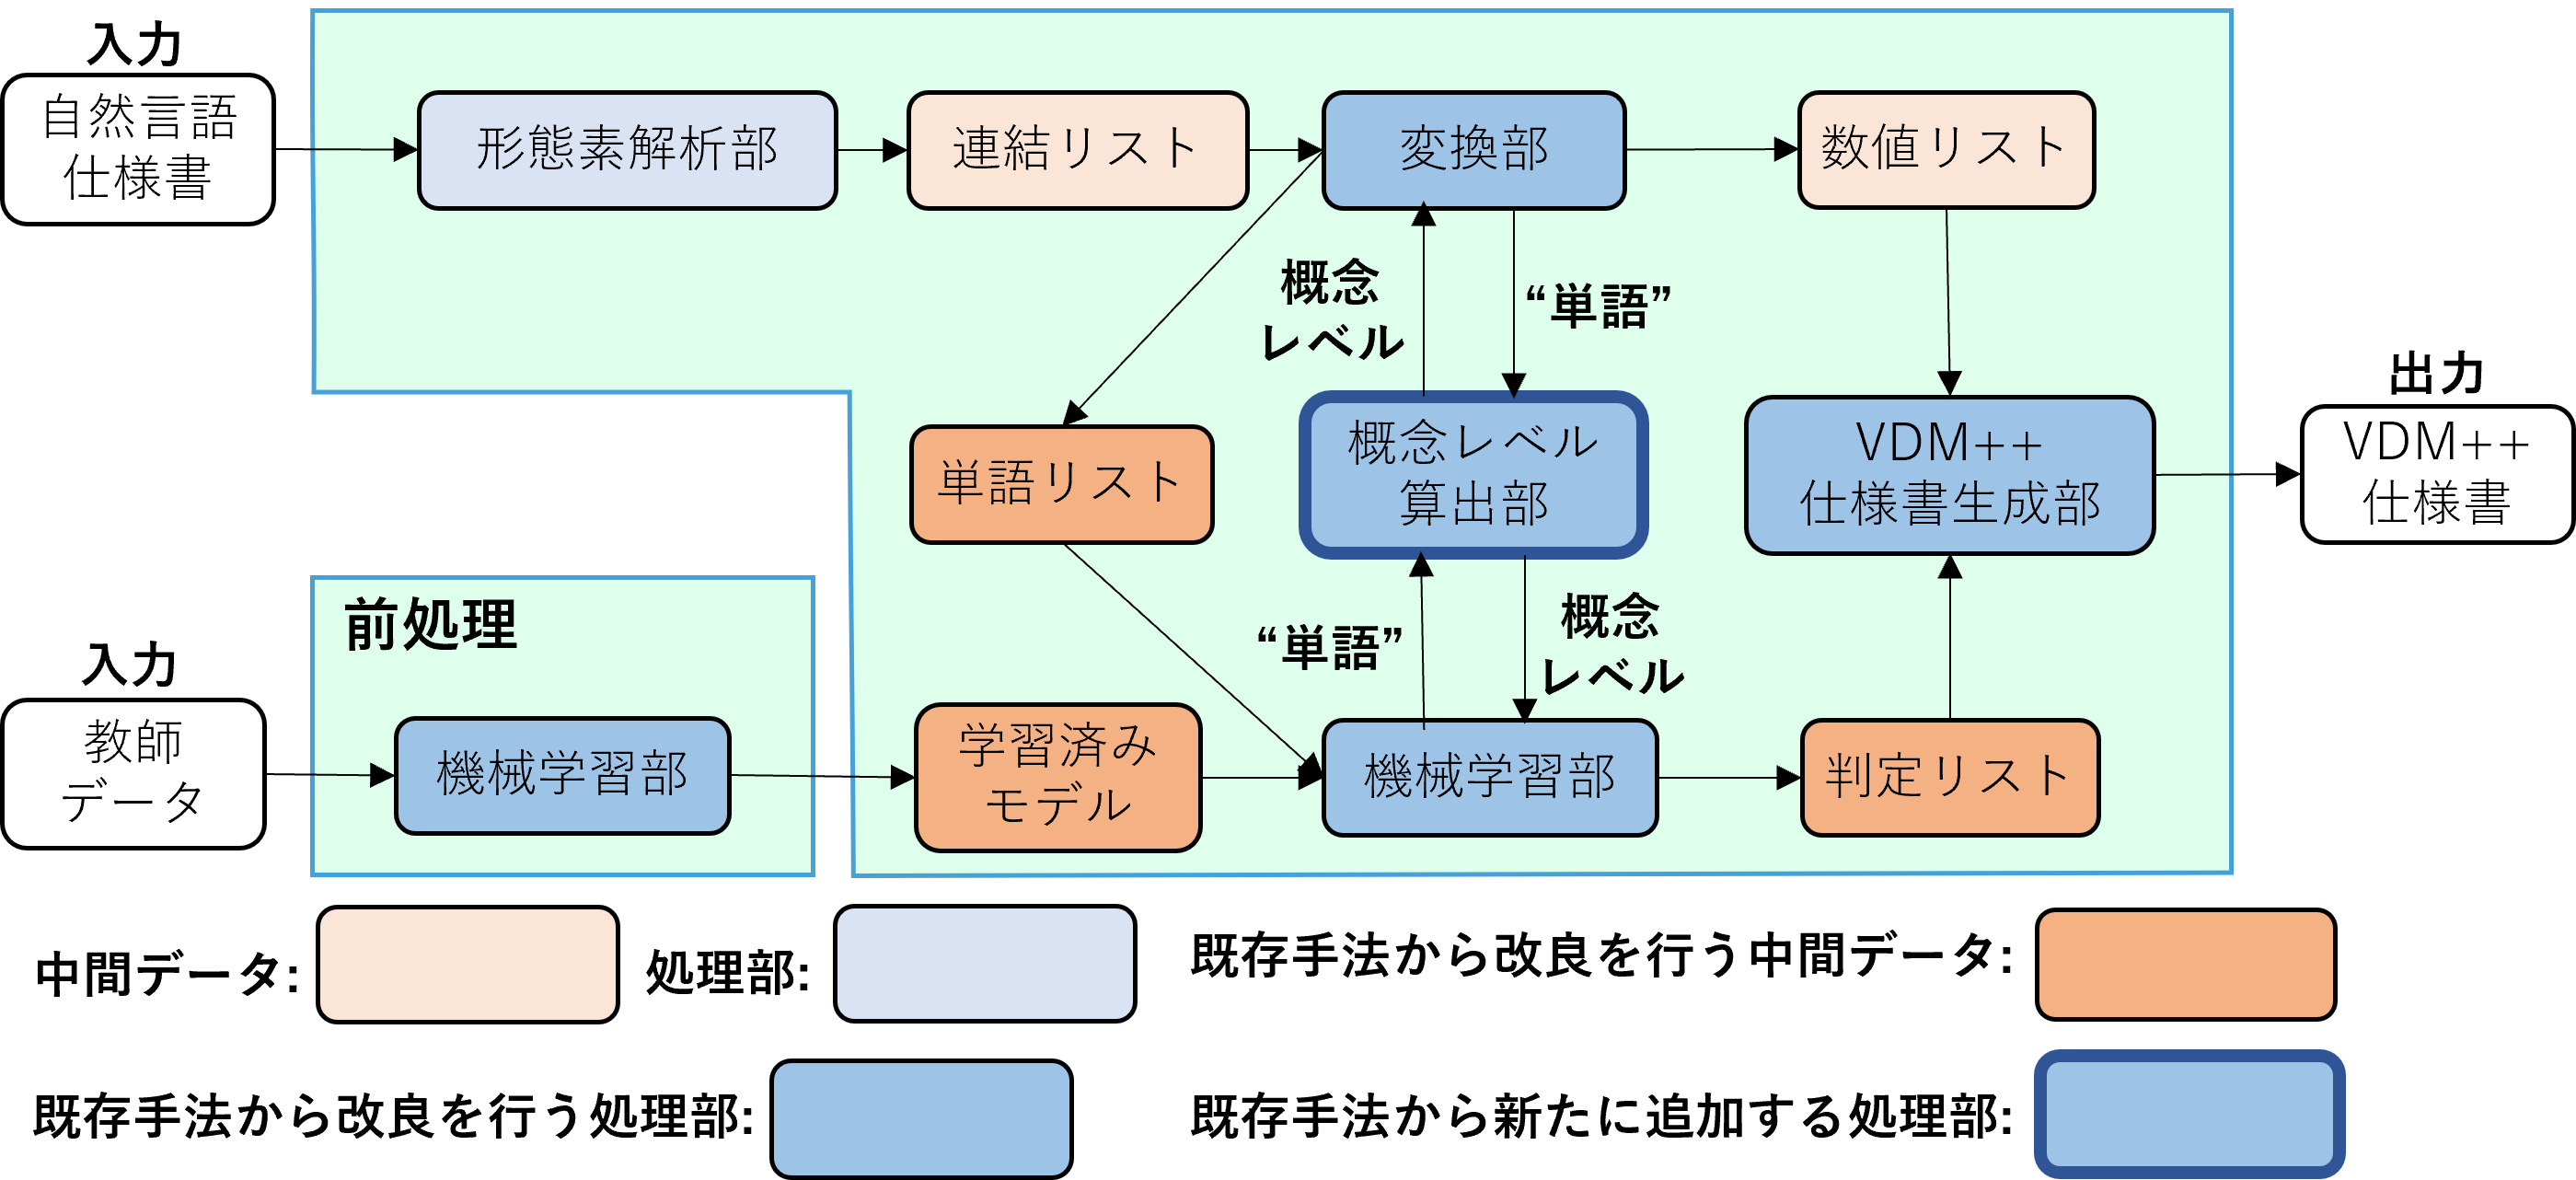
\includegraphics[width=1.0\columnwidth]{image/vgml_structure.png}
        \caption{VGMLの構造}
        \label{fig:vgml_structure}
    \end{center}
\end{figure}

\section{自然言語仕様書内の分かち書きした単語を連結する処理の改良}
本節では、自然言語仕様書内の分かち書きした単語を連結する処理の改良について説明する。
具体的には、既存手法の形態素解析部における単語連結処理を改良する。
VGMLの形態素解析部の構造を、図\ref{fig:vgml_mor_structure}に示す。

\begin{figure}[t]
    \begin{center}
        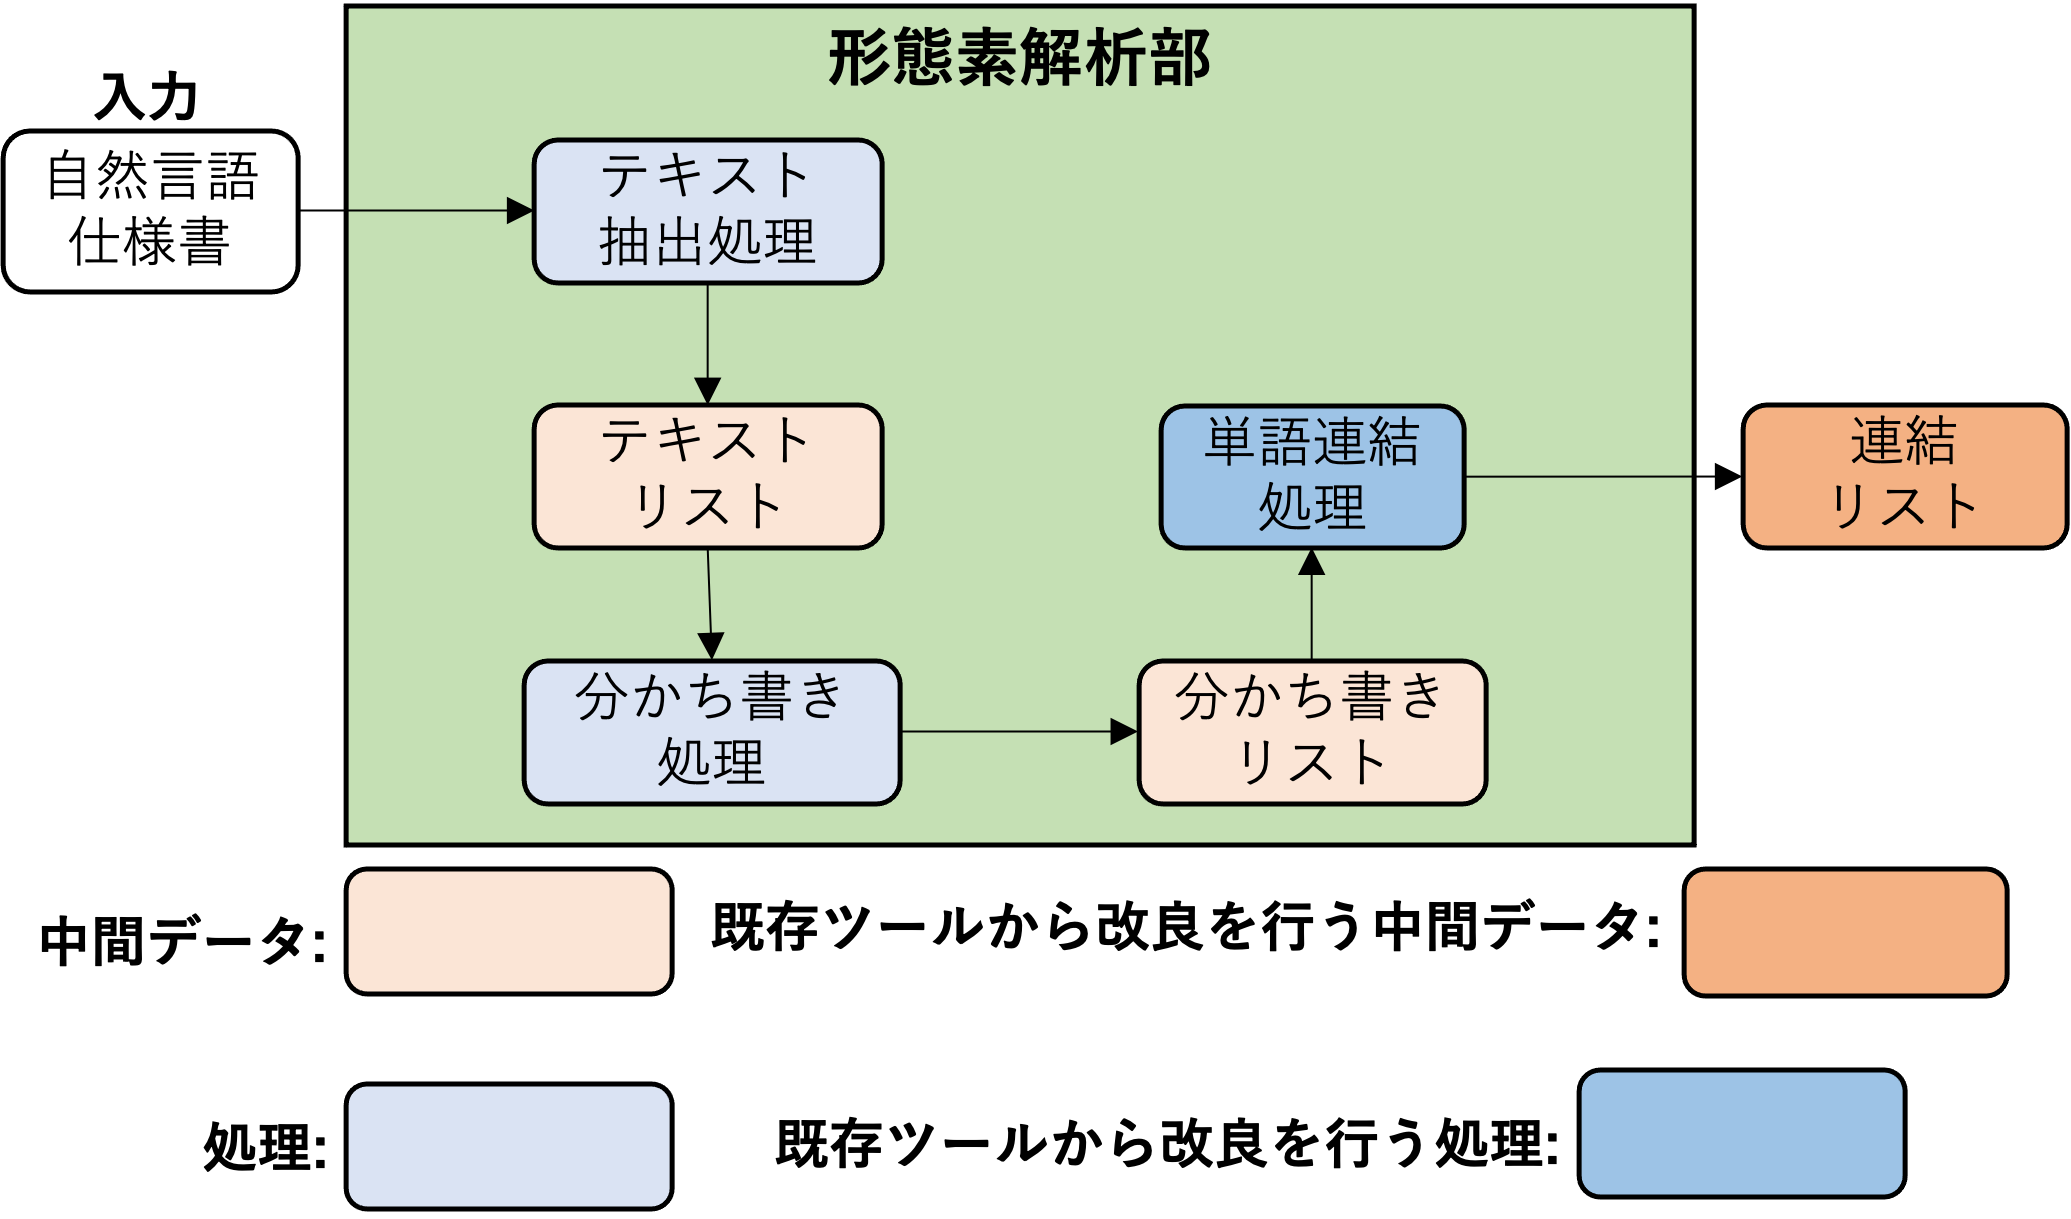
\includegraphics[width=1.0\columnwidth]{image/vgml_mor_structure.png}
        \caption{VGMLの形態素解析部の構造}
        \label{fig:vgml_mor_structure}
    \end{center}
\end{figure}

既存手法の形態素解析部における単語連結処理は、分かち書きリストを入力として読み込み、分かち書きリスト内の単語から助詞、助動詞、接続詞、副詞
の品詞である単語を除く。さらに、連続する2つ以上の名詞または動詞を連結し、連結した単語を格納した連結リストを生成する。
既存手法とVGMLの単語連結処理が入力とする分かち書きリストの例を、図\ref{fig:exis_wakati}に、既存手法の単語連結処理が出力する連結リストの例を、図\ref{fig:exis_connect}に示す。
図\ref{fig:exis_wakati}に示す分かち書きリストを分かち書き処理に入力した場合、図\ref{fig:exis_connect}に示すように、「企業」、「一覧」、「確認」を別の単語として出力する。
そのため、「企業の一覧を確認する」という意味を持つ単語を抽出することができない。
したがって、自然言語仕様書から抽出した単語をVDM++仕様書に記述する際に、各構文に対して適切な単語を記述することができない。

\begin{figure}[t]
    \begin{center}
        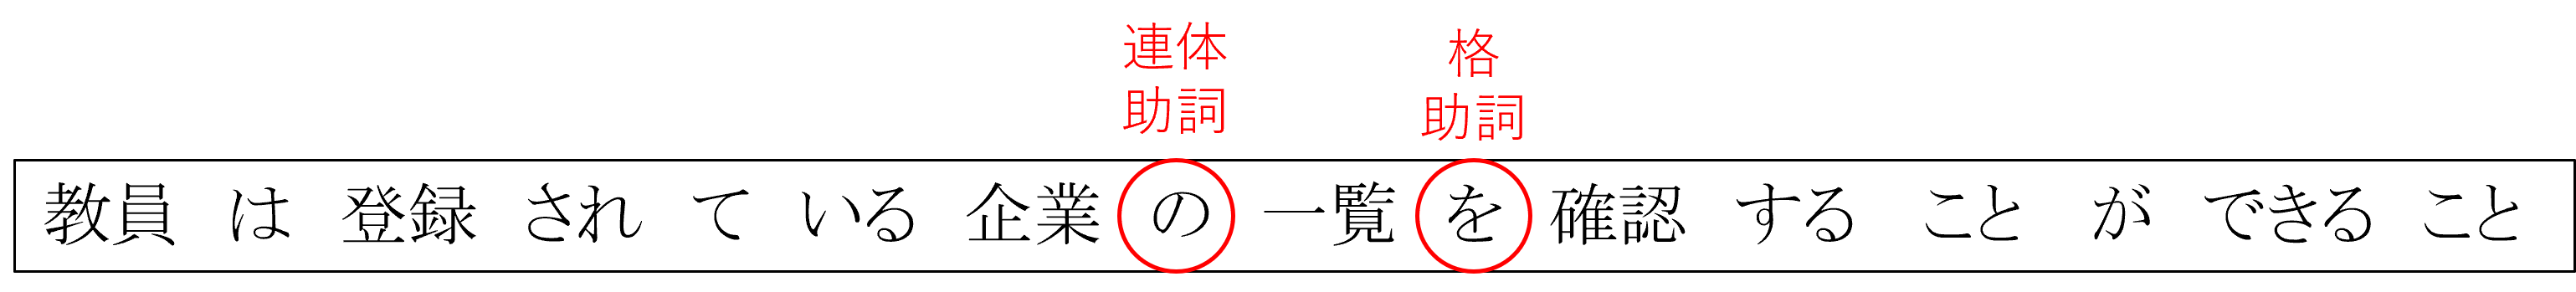
\includegraphics[width=1.0\columnwidth]{image/exis_wakati.png}
        \caption{既存手法とVGMLの単語連結処理が入力とする分かち書きリストの例}
        \label{fig:exis_wakati}
    \end{center}
\end{figure}

\begin{figure}[t]
    \begin{center}
        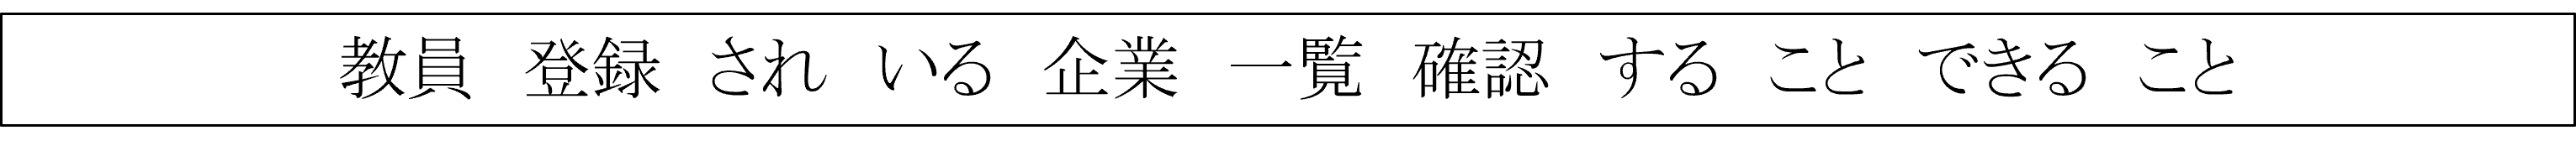
\includegraphics[width=1.0\columnwidth]{image/exis_connect.png}
        \caption{既存手法の単語連結処理が出力する連結リストの例}
        \label{fig:exis_connect}
    \end{center}
\end{figure}

\begin{figure}[t]
    \begin{center}
        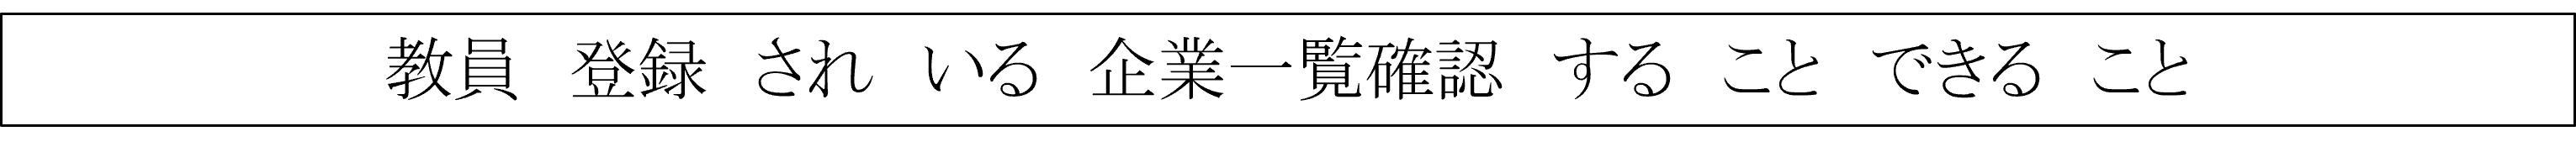
\includegraphics[width=1.0\columnwidth]{image/vgml_connect.png}
        \caption{VGMLの単語連結処理が出力する連結リストの例}
        \label{fig:vgml_connect}
    \end{center}
\end{figure}

VGMLの形態素解析部における単語連結処理は、既存手法が除く品詞が助詞である分かち書きリスト内の単語の内、連体助詞と格助詞に接続する2つの名詞を連結することによって、
上記の問題を解決する。
図\ref{fig:exis_wakati}に示す分かち書きリストを入力として、VGMLの単語連結処理が生成する連結リストの例を、図\ref{fig:vgml_connect}に示す。
図\ref{fig:vgml_connect}に示すように、VGMLの単語連結処理は、連体助詞と格助詞に接続する「企業」と「一覧」、「一覧」と「確認」を連結する。
そのため、「企業の一覧を確認する」という意味を持つ「企業一覧確認」という単語を抽出することができる。

\section{クラスを生成する処理の追加}
\label{sec:generate_class}
本節では、自然言語仕様書からVDM++仕様書におけるクラスを生成する手法について説明する。具体的には、既存手法に対して以下の処理部の追加と、処理の改良を行う。

\begin{itemize}
    \item 本論文で新たに定義する概念レベルの算出処理部の追加。
    \item 変換部の自然言語仕様書内の単語にパラメータを追加する処理の改良。
    \item 機械学習部の学習済みモデルを生成する処理の改良。
    \item 機械学習部の自然言語仕様書内の単語を分類する処理の改良。
    \item VDM++仕様書生成部にクラス分類処理の追加。
\end{itemize}

以降、4つの追加した処理部と、改良した処理について詳細を述べる。

\subsection{概念レベルの算出処理部の追加}
\label{sec:part_calc_concept_level}
既存手法は、機械学習に必要なパラメータとして、各単語に\ref{}節で述べたTF-IDF値、出現回数、優先値、連結回数の4つの値を追加する。
また、これらのパラメータを用いた機械学習によって自然言語内の単語を、VDM++仕様書に必要である単語と、必要でない単語に分類することができる。

VGMLは、機械学習に必要なパラメータとして、各単語にTF-IDF値、出現回数、優先値、連結回数に加えて、本論文で新たに定義する概念レベルを追加する(\ref{sec:improve_word_list}節に後述)。
これにより、機械学習によって自然言語仕様書内の単語を、以下の3つに分類することができる。

\begin{itemize}
    \item VDM++仕様書に必要でない単語
    \item VDM++仕様書に必要であるが、クラスの候補ではない単語
    \item VDM++仕様書に必要であり、かつ、クラスの候補である単語
\end{itemize}

以降、VDM++仕様書に必要でない単語をUNNECESSARY、VDM++仕様書に必要であるが、クラスの候補ではない単語をNONCLASS、
VDM++仕様書に必要であり、かつ、クラスの候補である単語をCLASSとそれぞれ表現する。

概念レベルの計算は、\ref{}節で述べた日本語WordNetを用いて、解析対象である単語の同義語とその下位概念の関係を表す木構造を生成する。
単語の下位概念の関係を表す木構造の例を、図\ref{fig:tree_structure}に示す。図\ref{fig:tree_structure}は、"りんご"の文字列を入力した際の木構造の例である。
日本語WordNetは、日本語での入力に対応しているが、出力する概念を表す単語は英語表記であるため、木構造を構成する単語も英語表記となる。
図\ref{fig:tree_structure}の木構造の場合、りんごの概念を持つ同義語を最上位のノードとし、その下位概念である単語を子ノードとして表現する。
概念レベル算出部の構造を、図\ref{fig:vgml_concept_level_structure}に示す。
概念レベル算出部の同義語検索処理は、入力として受け取った単語と同じ概念を持つ単語を検索し、検索した単語を格納した同義語リストを生成する。
概念レベル算出部は、1つの単語を入力として読み込み、算出した概念レベルを返す。
概念レベル算出部の処理の流れの例を図\ref{fig:flow_calc_concept_level}に、概念レベル算出部の処理の流れの説明を以下に示す。

\begin{figure}[t]
    \begin{center}
        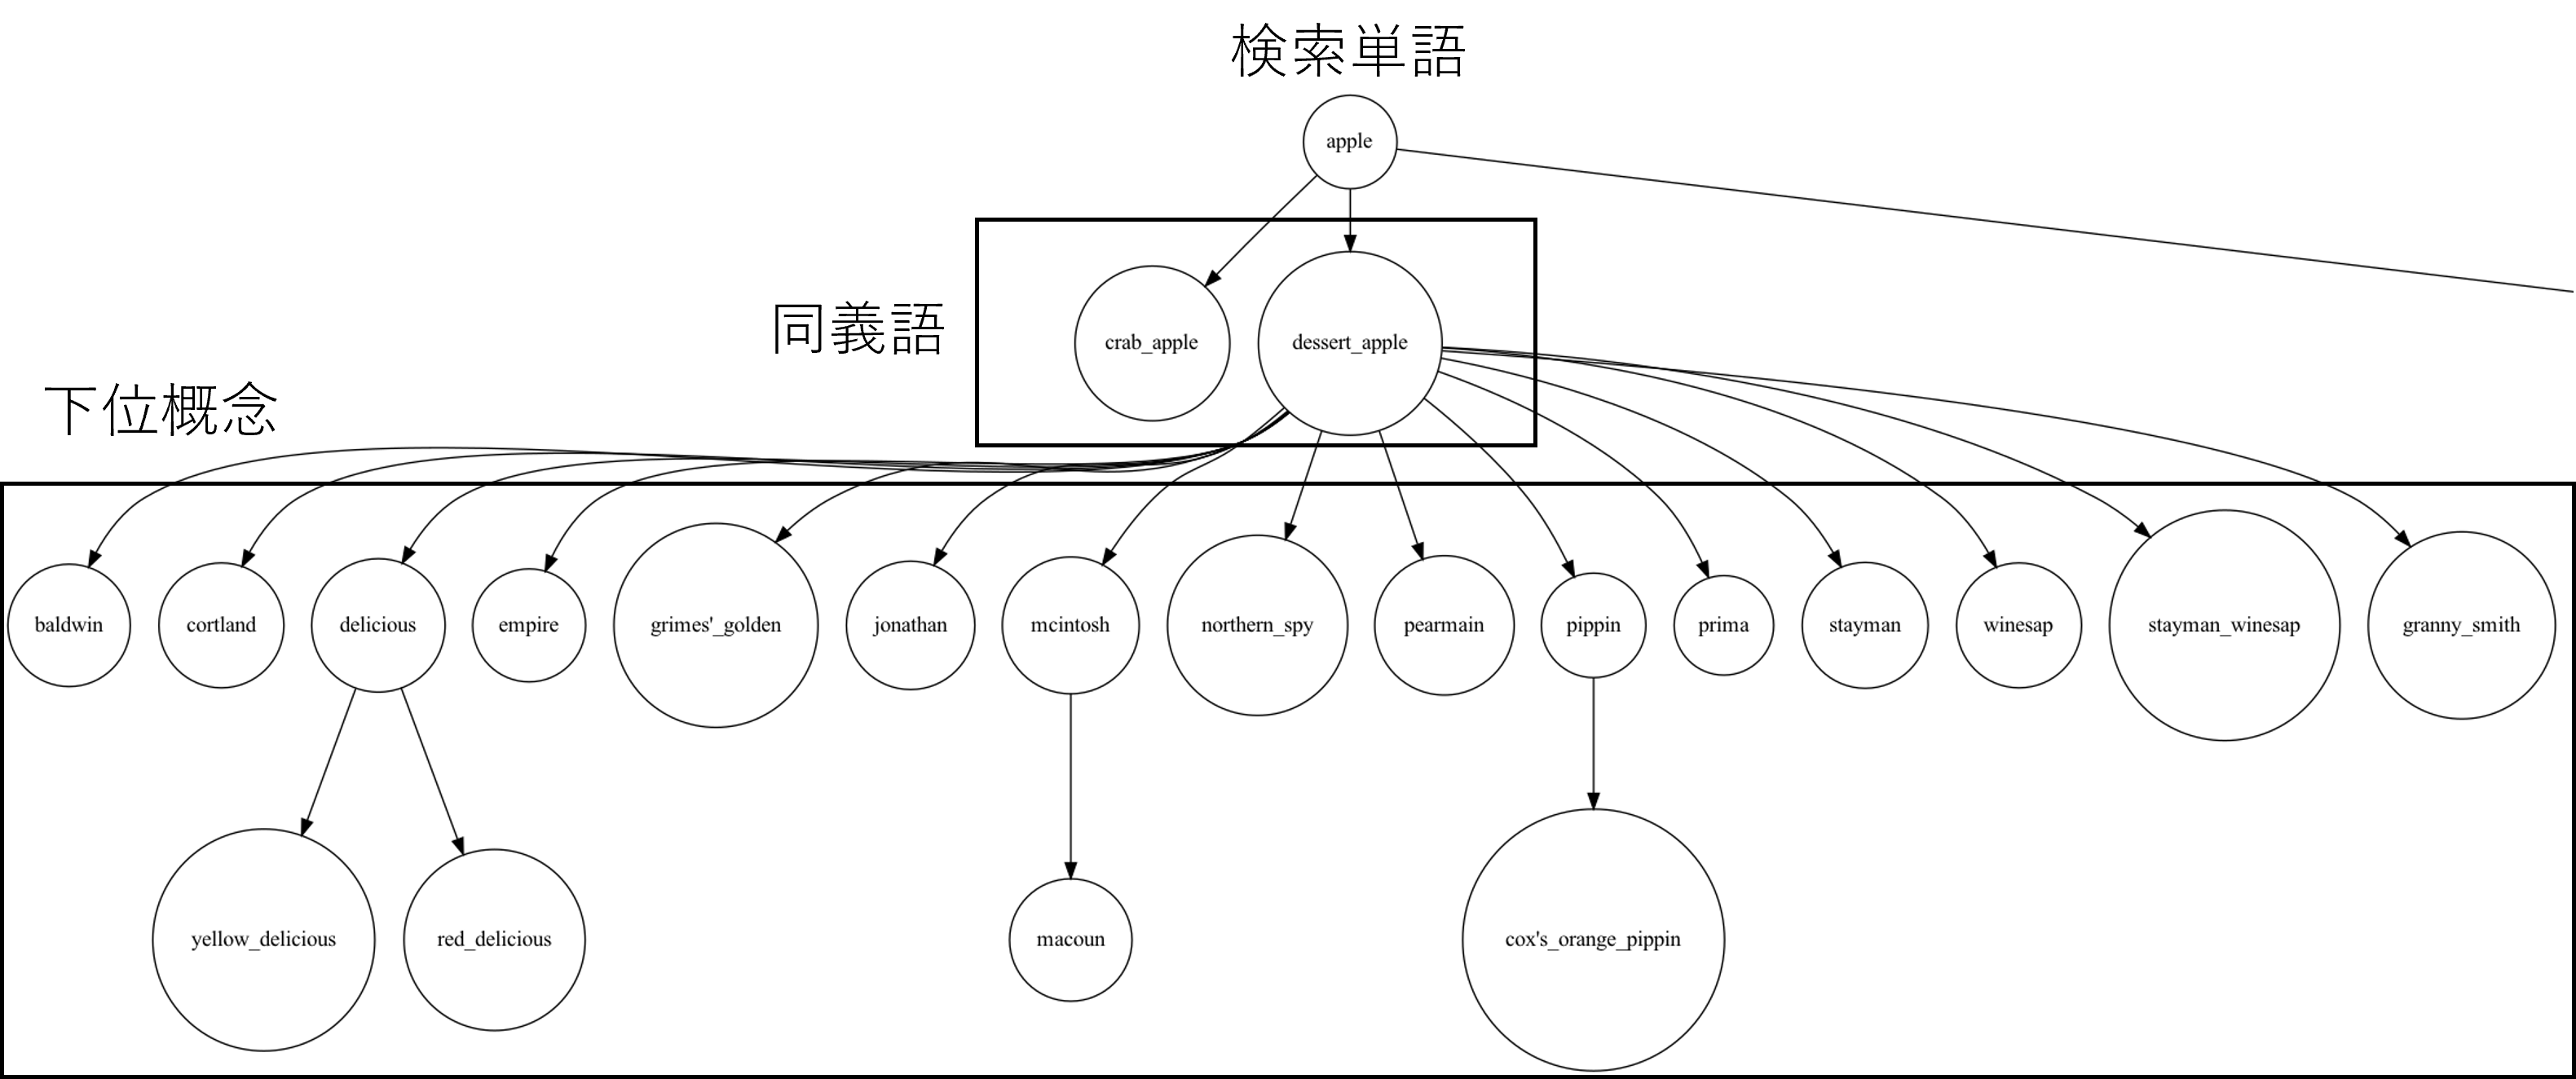
\includegraphics[width=1.0\columnwidth]{image/tree_structure.png}
        \caption{``りんご''を入力した際の下位概念の関係を表す木構造の例}
        \label{fig:tree_structure}
    \end{center}
\end{figure}

\begin{figure}[t]
    \begin{center}
        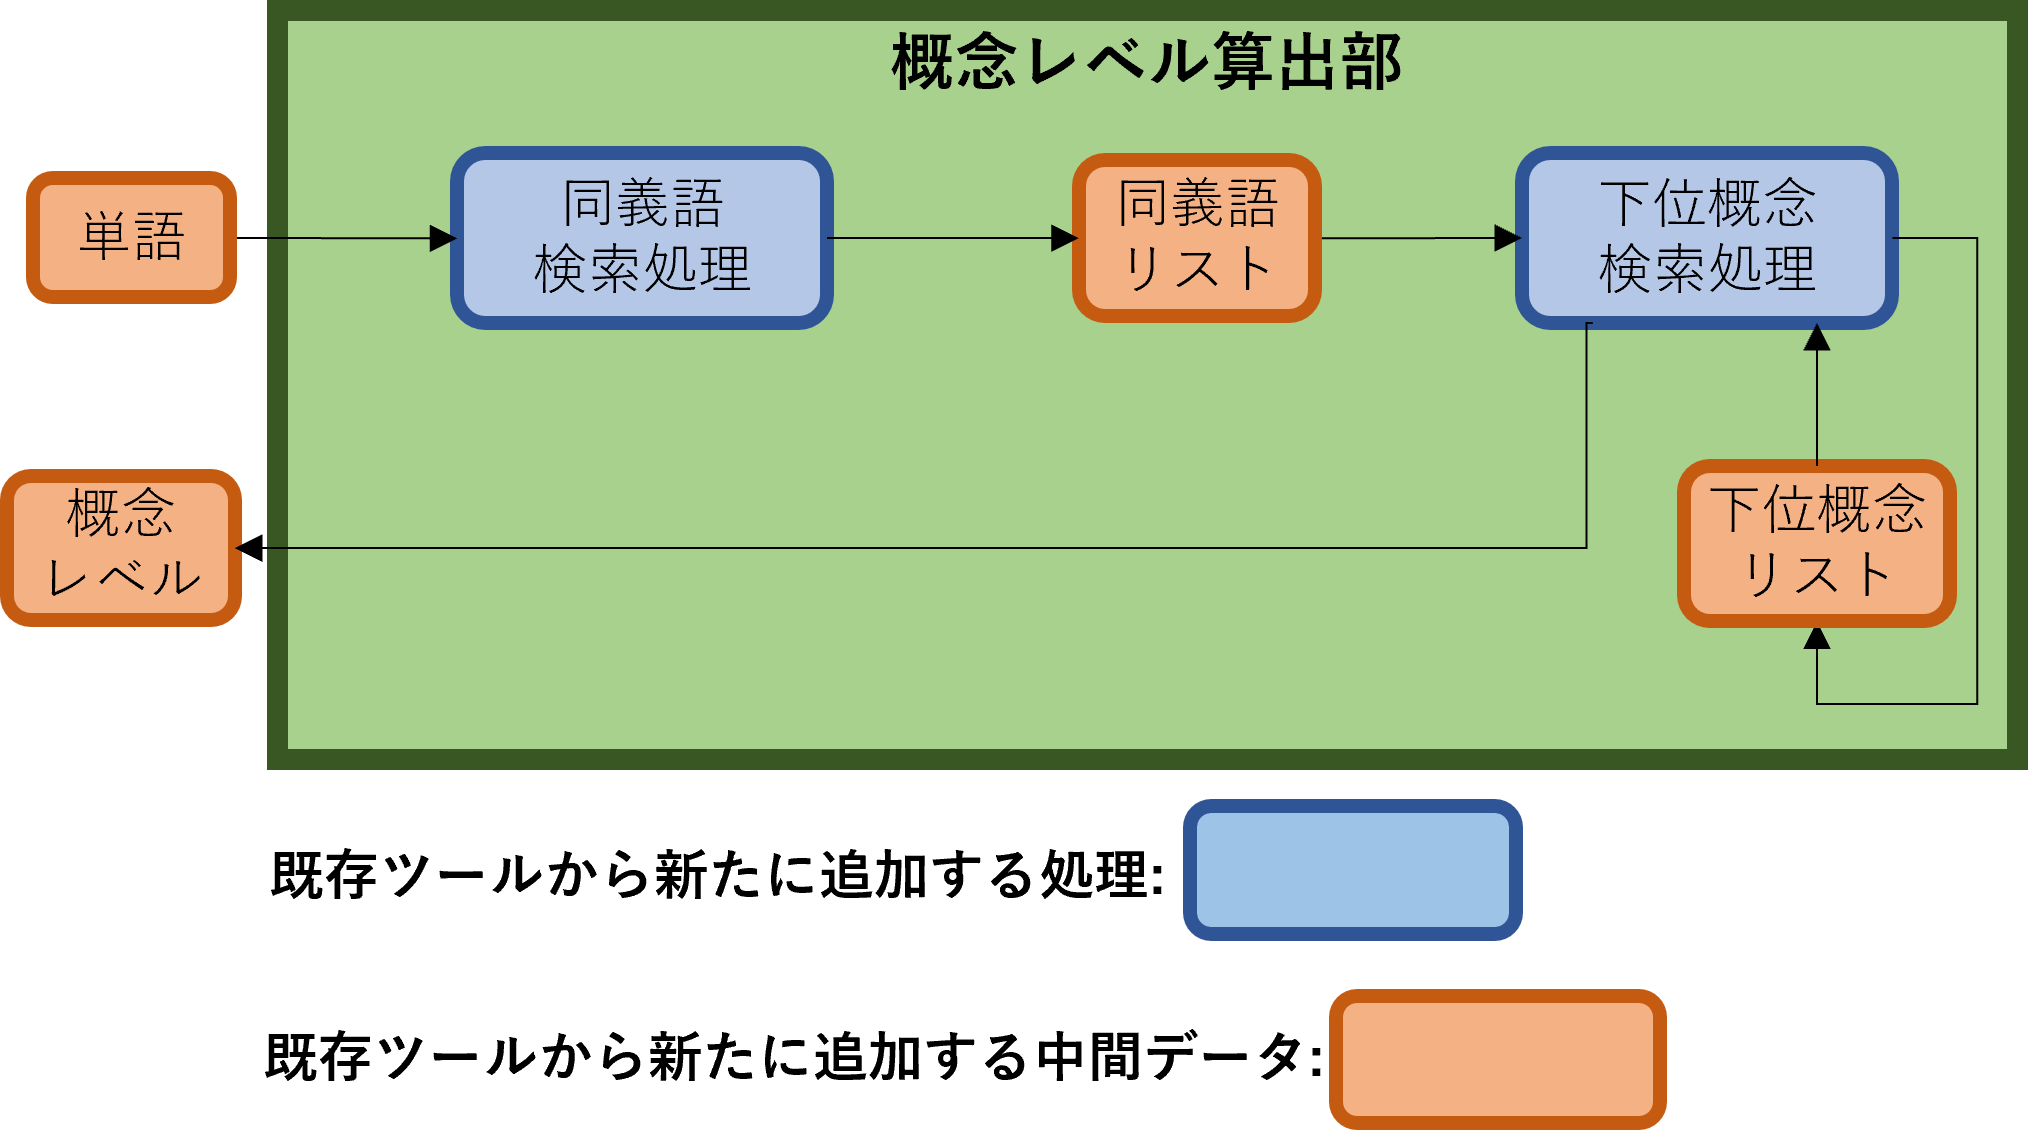
\includegraphics[width=1.0\columnwidth]{image/vgml_concept_level_structure.png}
        \caption{概念レベル算出部の構造}
        \label{fig:vgml_concept_level_structure}
    \end{center}
\end{figure}

\begin{figure}[t]
    \begin{center}
        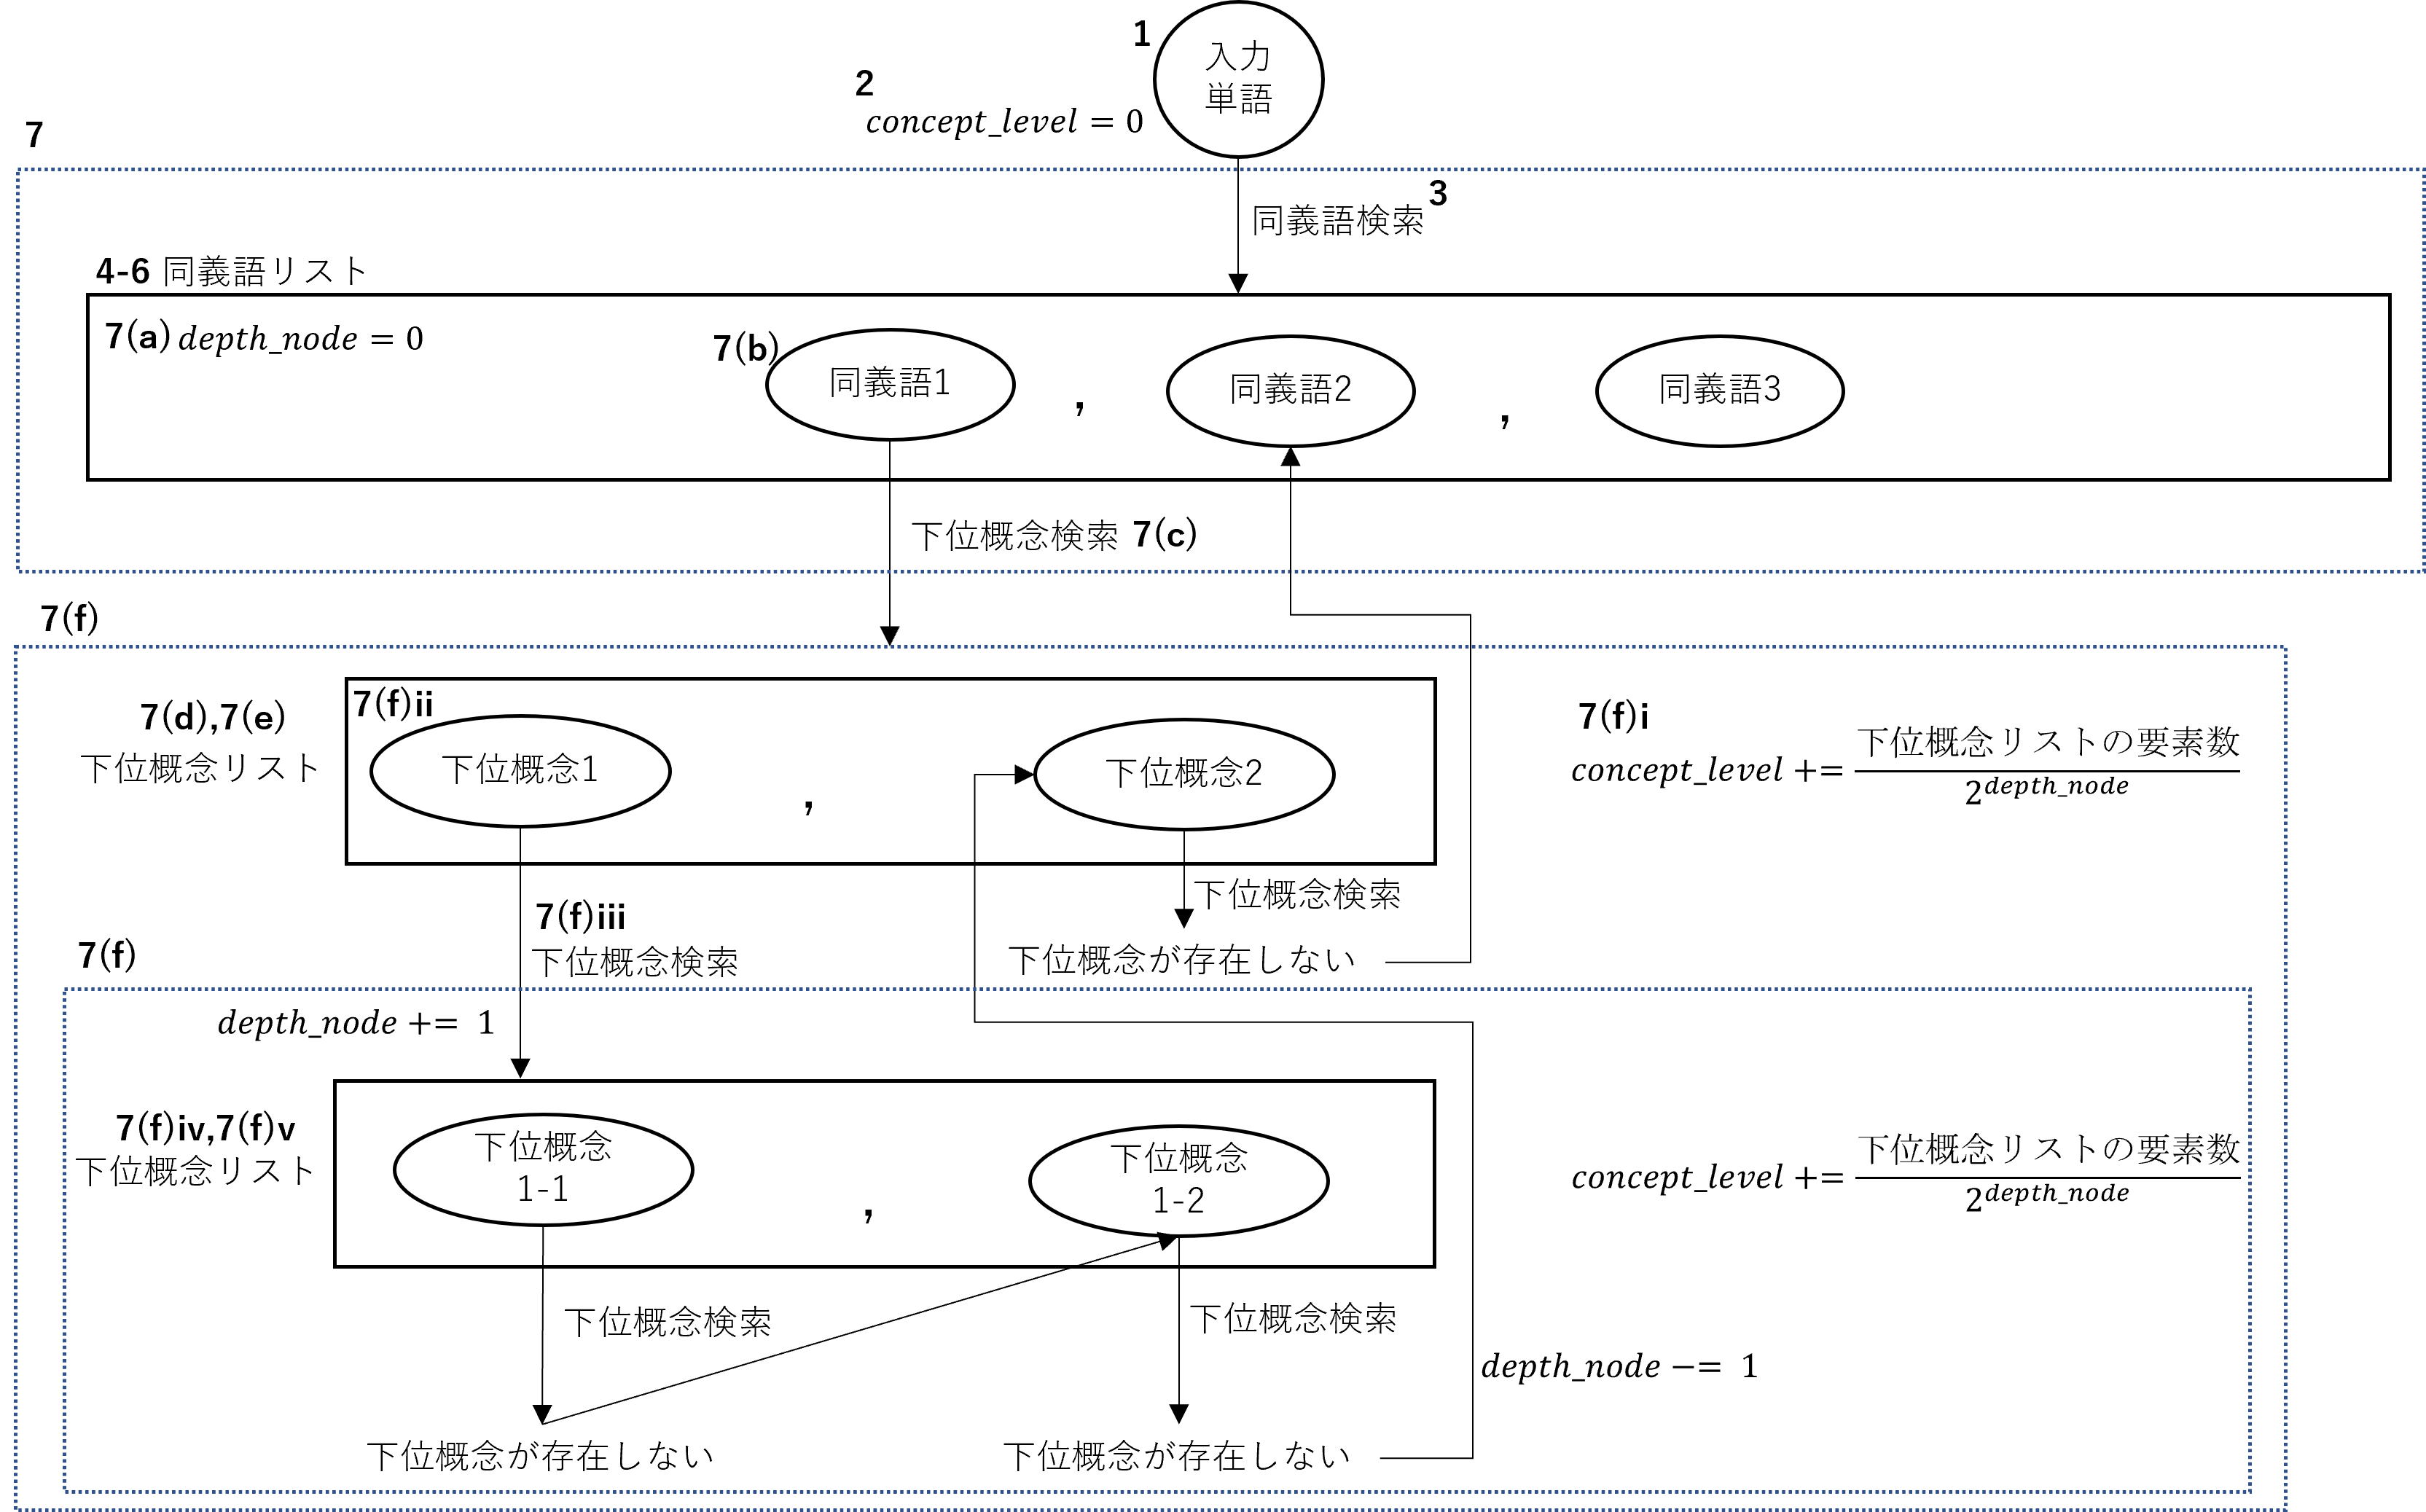
\includegraphics[width=1.0\columnwidth]{image/flow_calc_concept_level.png}
        \caption{概念レベル算出部の処理の流れの例}
        \label{fig:flow_calc_concept_level}
    \end{center}
\end{figure}

\begin{enumerate}
    \item 同義語検索処理は、単語を入力として読み込む。
    \label{sec:input_word}
    \item 同義語検索処理は、変数$concept\_level$を、0を初期値として定義する。変数$concept\_level$は、概念レベルを表す。
    \item 同義語検索処理は、日本語WordNetから\ref{sec:input_word}で入力した単語の同義語を検索する。
    \label{search_dogigo}
    \item 同義語検索処理は、空のリストを用意する。
    \label{sec:synonym_list}
    \item \ref{search_dogigo}で検索した同義語を\ref{sec:synonym_list}で用意した空のリストに格納する。このリストを、以降、同義語リストと表現する。同義語が存在しない場合、概念レベルを0として返して処理を終了する。
    \item 同義語検索処理は、同義語リストを下位概念検索処理に渡す。
    \item 下位概念検索処理は、同義語リストの要素の数だけ以下の処理を繰り返す。
        \begin{enumerate}
            \item 変数$depth\_node$を、0を初期値として定義する。変数$depth\_node$は、単語の上位下位の関係を表す木構造における、ノードの深さを表す。
            \label{sec:loop_synonym_list}
            \item 同義語リストから、同義語を表す単語を1つ読み込む。
            \label{sec:read_synonym_word}
            \item 日本語WordNetから\ref{sec:read_synonym_word}で読み込んだ単語の下位概念を検索する。
            \item 空のリストを用意する。
            \label{sec:lower_concept_list}
            \item 検索した下位概念を\ref{sec:lower_concept_list}で用意した空のリストに格納する。このリストを、以降、下位概念リストと表現する。下位概念が存在しない場合、\ref{sec:loop_synonym_list}に戻る。
            \item 下位概念リストの要素の数だけ以下の処理を再帰的に繰り返す。
                \begin{enumerate}
                    \item $concept\_level$に$(下位概念リストの要素数\quad/\quad2^{depth\_node})$の値を加える。
                    \label{sec:loop_lower_list}
                    \item 下位概念リストから、下位概念を表す単語を1つ読み込む
                    \label{sec:read_lower_word}
                    \item 日本語WordNetから\ref{sec:read_lower_word}で読み込んだ単語の下位概念を検索する。
                    \item 空のリストを用意する
                    \label{sec:lower_concept_list2}
                    \item 検索した下位概念を\ref{sec:lower_concept_list2}で用意した空のリストに格納する。
                    \label{sec:update_lower_concept_list}
                    \item \ref{sec:update_lower_concept_list}のリストに対し以下のいずれかの処理を行う。
                    \begin{itemize}
                        \item \ref{sec:update_lower_concept_list}のリストが空ではない、つまり、下位概念が存在する場合、\ref{sec:update_lower_concept_list}のリストを下位概念リストとし、$depth\_node$に1を加えて\ref{sec:loop_lower_list}に戻る。
                        \item \ref{sec:update_lower_concept_list}のリストが空である、つまり、下位概念が存在しない場合、\ref{sec:loop_lower_list}に戻る。
                        \item \ref{sec:update_lower_concept_list}のリストが空である、つまり、下位概念が存在しない、かつ、\ref{sec:read_lower_word}で読み込んだ単語が下位概念リストの末尾の要素である場合、$depth\_node$から1を引いて\ref{sec:loop_lower_list}に戻る。
                    \end{itemize}
                \end{enumerate}
        \end{enumerate}
\end{enumerate}

\subsection{自然言語仕様書内の単語にパラメータを追加する処理の改良}
\label{sec:improve_word_list}
既存手法は、図\ref{}に示す変換部において、各単語にTF-IDF値、出現回数、優先値、連結回数の4つの値を追加する。
さらに、図\ref{}に示す単語リストを生成する。
既存手法が生成する単語リストは、単語名と、各単語に対して算出した、TF-IDF値、出現回数、優先値、連結回数の4つのパラメータを持つ。

VGMLの変換部の構造を図\ref{fig:vgml_transfer}に、VGMLが生成する単語リストの例を図\ref{fig:vgml_word_list}にそれぞれ示す。
VGMLの変換部における概念レベル生成処理は、図\ref{}に示す既存手法が生成する連結リストを、列数5の一時ファイルとして入力する。
さらに、\ref{sec:part_calc_concept_level}節で述べた様に、図\ref{fig:vgml_concept_level_structure}に示す概念レベル算出部において、本論文で新たに定義する概念レベルを計算する。
最後に、変換部の概念レベル生成処理において、列数5の一時ファイルに概念レベルを追加することによって、図\ref{fig:vgml_word_list}に示す単語リストを生成する。
VGMLが生成する単語リストは、単語名と、各単語に対して算出した、TF-IDF値、出現回数、優先値、連結回数、概念レベルの5つのパラメータを持つ。

以降、VGMLの変換部における概念レベル生成処理の流れを以下に示す。

\begin{enumerate}
    \item 列数5の一時ファイルを入力として読み込む。
    \label{sec:row5_file}
    \item 列数5の一時ファイルの行の数だけ、以下の処理を繰り返す。
        \begin{enumerate}
            \item 1列目の連結リストの単語を読み込む。
            \label{sec:search_concept_word}
            \item \ref{sec:part_calc_concept_level}節で述べた概念レベル算出部において、\ref{sec:search_concept_word}で読み込んだ単語を入力とし、概念レベルを計算する。
            \label{sec:generate_concept_level}
            \item \ref{sec:generate_concept_level}で計算した値を、\ref{sec:row5_file}で読み込んだ列数5の一時ファイルの同じ行の末尾に新たな要素として追加する。
        \end{enumerate}
\end{enumerate}

この列数5の一時ファイルの末尾に新たな要素を追加した1行は、(連結リストの単語、TF-IDF値、出現回数、優先値、連結回数、概念レベル)で構成する。
このファイルが、図\ref{fig:vgml_word_list}に示す単語リストである。

図\ref{fig:vgml_word_list}に示すように、概念レベルの値と自然言語仕様書内の単語には、以下のような特徴が見られた。

\begin{itemize}
    \item 概念レベルの値が大きすぎる単語(``システム''など)は、VDM++仕様書に必要でない単語の可能性が高い。
    \item 概念レベルの値が小さすぎる単語 (``ID''、``パスワード''など)は、VDM++仕様書に必要でない単語である可能性が高い。しかし、クラスの候補となる単語に接続する場合、そのクラスが持つインスタンス変数となる可能性が高い。
    \item 大きすぎる概念レベルの値と、小さすぎる概念レベルの値の中間程度の概念レベルの値である単語(``企業''、``企業担当者''など)の内、概念レベルの値が大きい単語は、クラスの候補である単語の可能性が高い。
    \item 上記の項目にあてはまらない単語(``年度''など)は、クラスの候補でない単語の可能性が高い。
\end{itemize}

VGMLは、上記の特徴に基づいて、各単語をUNNECESSARY、NONCLASS、CLASSのいずれかに分類する。

\begin{figure}[t]
    \begin{center}
        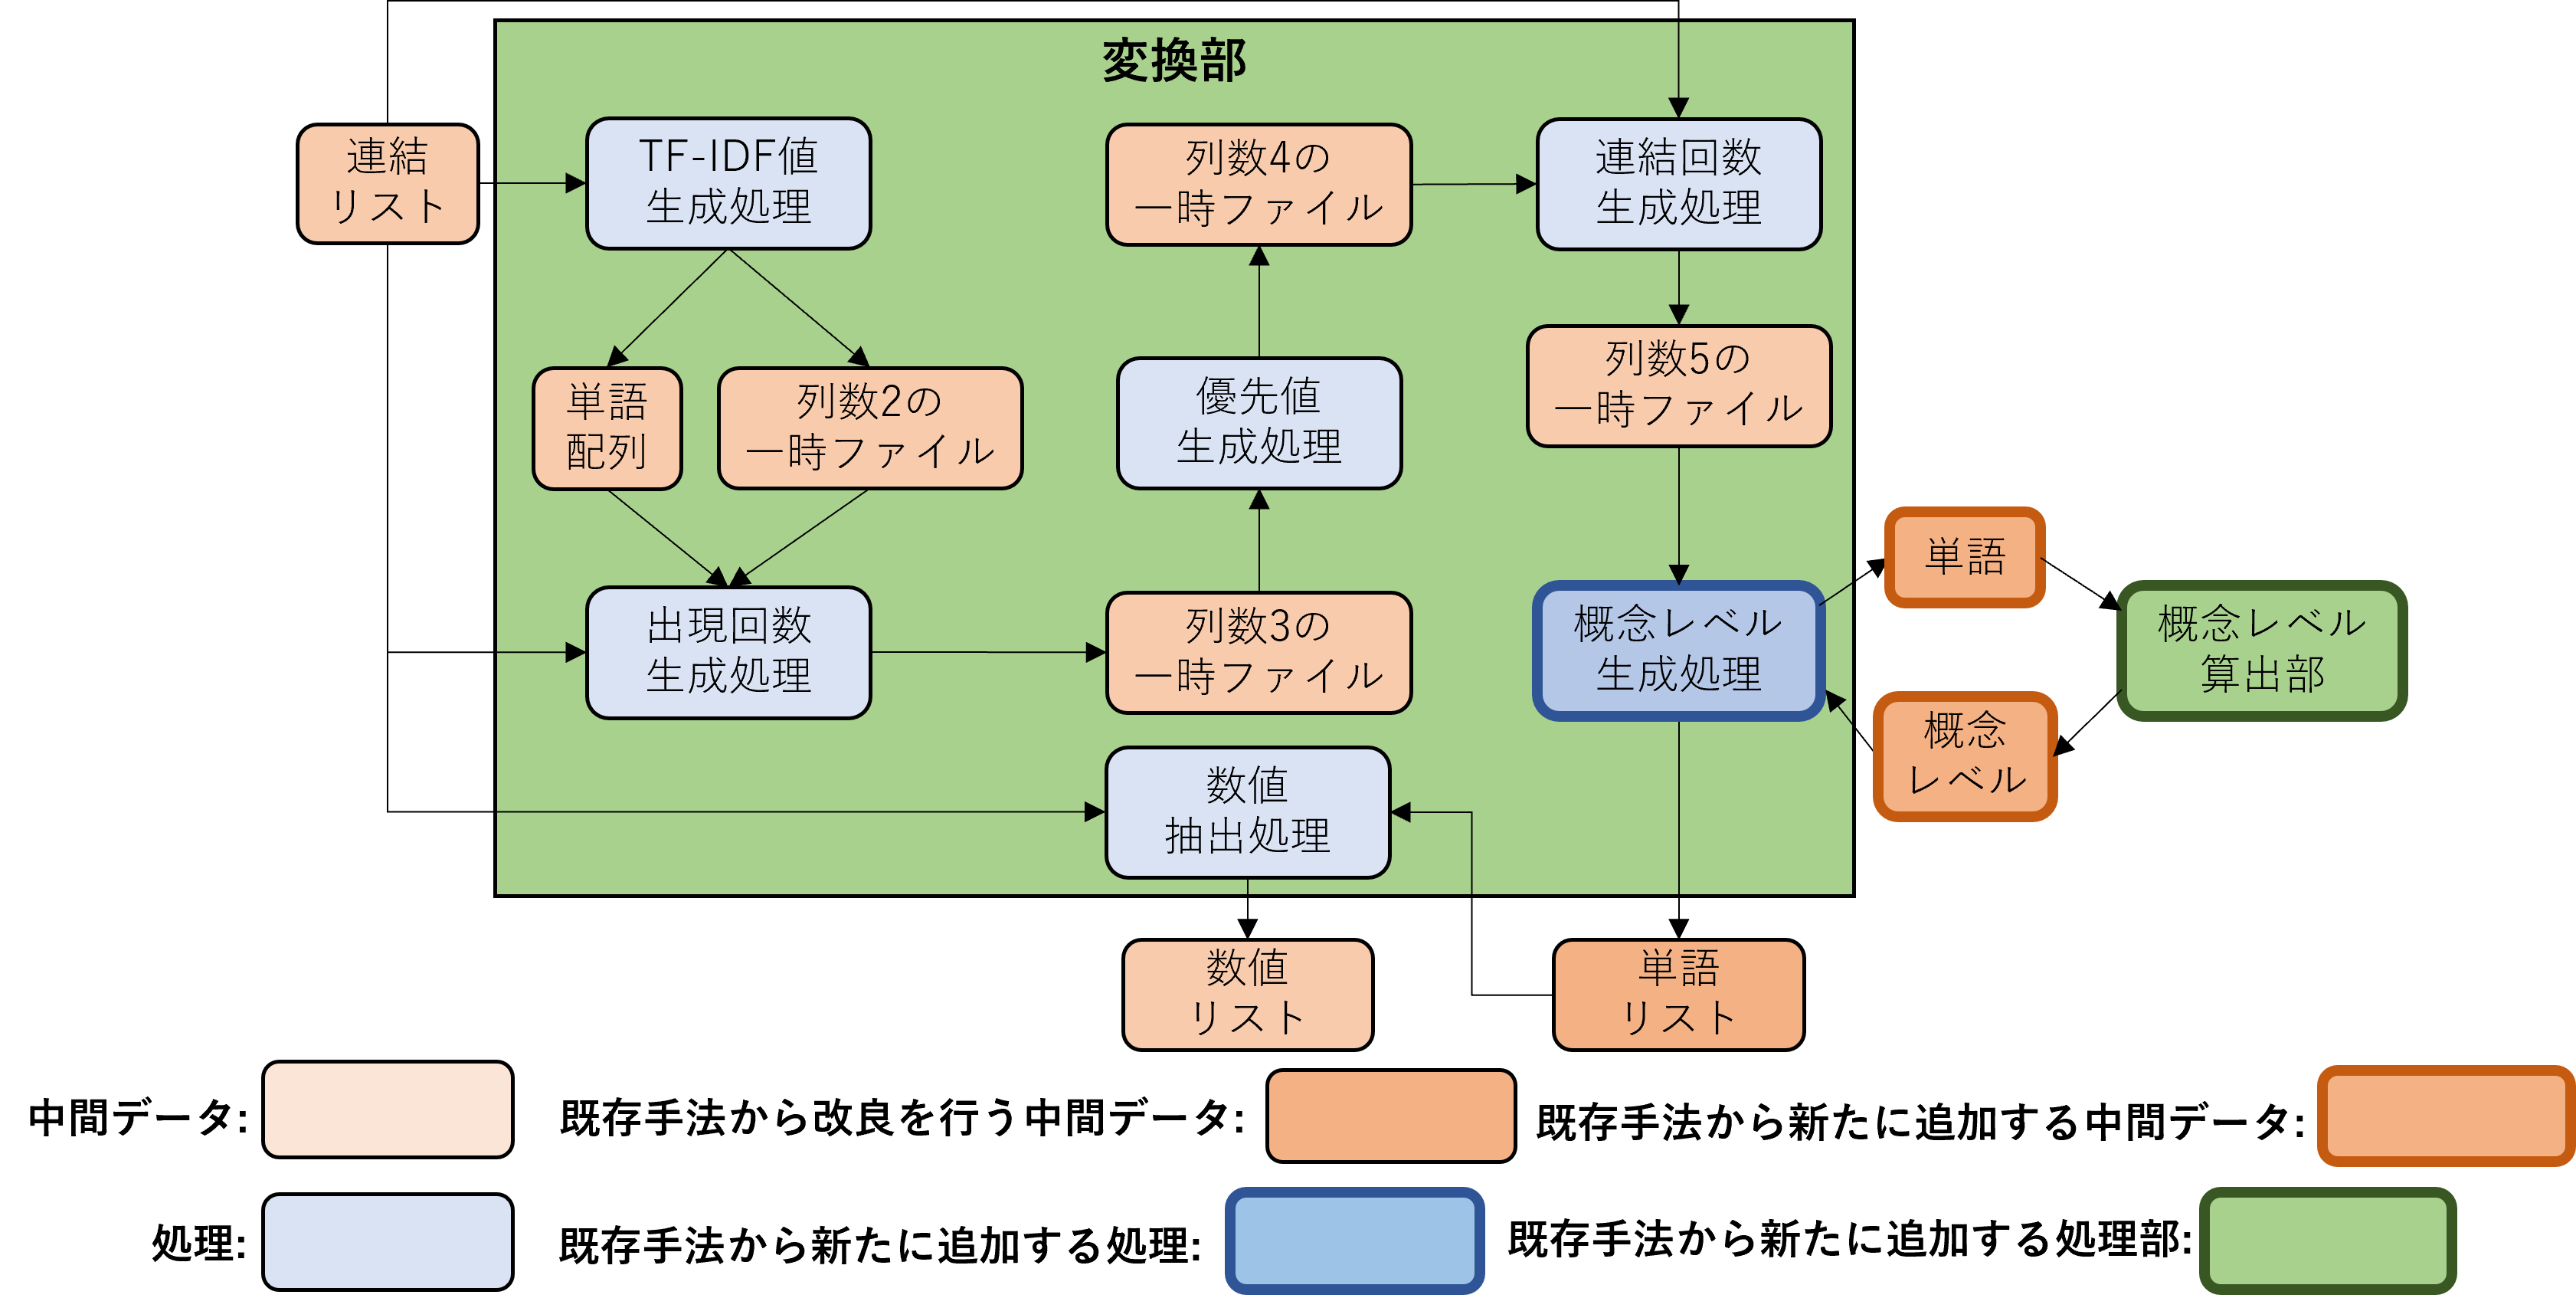
\includegraphics[width=1.0\columnwidth]{image/vgml_transfer.png}
        \caption{VGMLの変換部の構造}
        \label{fig:vgml_transfer}
    \end{center}
\end{figure}

\begin{figure}[t]
    \begin{center}
        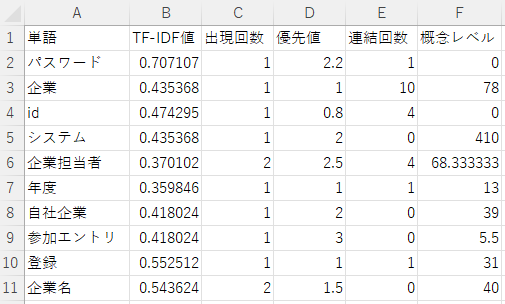
\includegraphics[width=1.0\columnwidth]{image/vgml_word_list.png}
        \caption{VGMLが生成する単語リストの例}
        \label{fig:vgml_word_list}
    \end{center}
\end{figure}

\subsection{機械学習部の学習済みモデルを生成する処理の改良}
\label{sec:vgml_train_model}
既存手法における教師データは、図\ref{fig:}に示すように、
1列目に単語名、2列目に判定結果、3列目以降に変換部で各単語に追加した TF-IDF値、出現回数、優先値、連結回数を説明変数として持つ。
判定結果は0か1のいずれかであり、0は1列目の単語がVDM++仕様書に必要でない単語であることを表し、
1は1列目の単語が VDM++仕様書に必要な単語であることを表す。
既存手法における前処理としての機械学習部は、自然言語仕様書内の単語を、VDM++仕様書に必要でない単語と、VDM++仕様書に必要な単語の2つの項目に分類するために、
図\ref{}に示す教師データを入力とし、\ref{sec:}節で述べた二項ロジスティック回帰分析を用いて学習済みモデルを生成する。

VGMLにおける教師データを、図\ref{fig:vgml_teach}に示す。
VGMLにおける教師データは、図\ref{}に示した既存手法の教師データに、\ref{sec:part_calc_concept_level}で述べた概念レベルを説明変数として追加する。
VGMLの教師データの判定結果はUNNECESSARY、NONCLASS、CLASS のいずれかである。
教師データの作成の際に、自然言語仕様書内の各単語に対し、以下のルールに従って人手で判定結果を与えた。

\begin{figure}[t]
    \begin{center}
        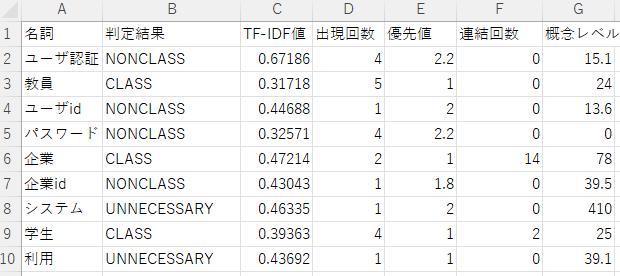
\includegraphics[width=1.0\columnwidth]{image/vgml_teach.png}
        \caption{VGMLにおける教師データ}
        \label{fig:vgml_teach}
    \end{center}
\end{figure}

\begin{itemize}
    \item CLASS
        \begin{itemize}
            \item 自然言語仕様書内で属性や振る舞いを持つ名詞であり、かつ、自然言語仕様書が対象とするシステムの外部に位置するアクターではない名詞。
        \end{itemize}
    \item NONCLASS
        \begin{itemize}
            \item あるクラスの候補となる名詞が持つ情報であり、かつ、自クラスまたは他のクラスの候補となる名詞が振る舞いを行う際に必要とする情報である名詞。
            \item あるクラスの候補となる名詞が行う振る舞いを表す名詞。
            \item システムで必要となる制約条件を表す名詞。
        \end{itemize}
    \item UNNECESSARY
        \begin{itemize}
            \item CLASSおよびNONCLASSのいずれにも属さない名詞。
        \end{itemize}
\end{itemize}

表\ref{table:data_set}に、教師あり学習のデータセット数を示す。

\begin{table}[t]
    \begin{center}
      \caption{教師データのデータセット数}
      \label{table:data_set}
      \begin{tabular}{c|c}
        データ総数 & 331\\
        \hline
        \hline
        CLASS    & 39\\ \hline
        NONCLASS & 157\\ \hline
        UNNECESSARY   & 135\\ \hline
      \end{tabular}
    \end{center}
  \end{table}

VGMLにおける前処理としての機械学習部は、自然言語仕様書内の単語を、UNNECESSARY、NONCLASS、CLASS のいずれかに分類するために、
図\ref{fig:vgml_teach}に示す教師データを入力とする。
さらに、\ref{sec:}節で述べた多項ロジスティック回帰分析を用いて学習済みモデルを生成する。

VGMLにおける学習済みモデル生成処理の流れを以下に示す。

\begin{enumerate}
	\item 教師データを、入力として読み込む。
    \label{teach_1}
	\item \ref{teach_1}で読み込んだ教師データの行の数だけ、以下の処理を繰り返す。
        \begin{enumerate}
            \item \ref{teach_1}で読み込んだ教師データの判定結果がCLASSの場合は、教師データのTF-IDF値、出現回数、優先値、連結回数、概念レベルをCLASSの説明変数として、定数と偏回帰変数を学習する。
            \item \ref{teach_1}で読み込んだ教師データの判定結果がNONCLASSの場合は、教師データのTF-IDF値、出現回数、優先値、連結回数、概念レベルをNONCLASSの説明変数として、定数と偏回帰変数を学習する。
            \item \ref{teach_1}で読み込んだ教師データの判定結果がUNNECESSARYの場合は、教師データのTF-IDF値、出現回数、優先値、連結回数、概念レベルをUNNECESSARYの説明変数として、定数と偏回帰変数を学習する。
        \end{enumerate}
	\item 学習後に、定数と偏回帰変数をパラメータとして学習済みモデルを出力する。
\end{enumerate}

\subsection{自然言語仕様書内の単語を分類する処理の改良}
既存手法における機械学習部の判定リスト生成処理は、\ref{sec:}で述べたように、変換部で生成した単語リストを入力とし、
学習済みモデルを使用して判定リストを生成する。
既存手法における機械学習部の判定リスト生成処理が生成する判定リストは、図\ref{fig:}に示すように、各単語に対しVDM++仕様書に必要な単語であることを表す1、またはVDM++仕様書に必要でない単語であることを表す0のいずれかの値を持つ。

VGMLにおける機械学習部の判定リスト生成処理は、\ref{sec:improve_word_list}節で述べた単語リストを入力とし、
\ref{sec:vgml_train_model}節で述べた学習済みモデルを使用して判定リストを生成する。
VGMLが生成する判定リストは、単語リストの単語に対するUNNECESSAEY、NONCLASS、CLASSのいずれに属するかの判定結果と、
単語が各項目に属する確率を単語リストに追加したものである。
VGMLが生成する判定リストの例を、図\ref{fig:vgml_judge_list}に示す。
各項目に対する結果の確率は、入力である単語リストの各パラメータを、学習済みモデルを用いて出力した値である。

\begin{figure}[t]
    \begin{center}
        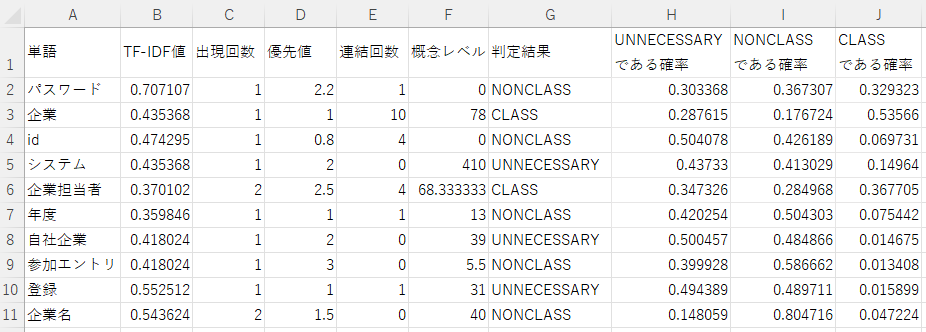
\includegraphics[width=1.0\columnwidth]{image/vgml_judge_list.png}
        \caption{VGMLが生成する判定リストの例}
        \label{fig:vgml_judge_list}
    \end{center}
\end{figure}

VGMLにおける機械学習部の判定リスト生成処理の流れを以下に示す。

\begin{enumerate}
    \item 単語リストを、入力として読み込む。
    \label{sec:read_word_list}
    \item \ref{sec:read_word_list}で読み込んだ単語リストの行の数だけ、以下の処理を繰り返す。
        \begin{enumerate}
            \item 単語リストのTF-IDF値、出現回数、優先値、連結回数、および、概念レベルを引数として、学習済みモデルを使用して各目的変数への確率を計算する。
            \label{sec:calc_probability}
            \item \ref{sec:calc_probability}で生成した各目的変数への確率を比較し、最も高い確率であるものを判定結果の項目とする。
            \item \ref{sec:read_word_list}で読み込んだ単語リストに、判定結果と確率を追加する。
        \end{enumerate}
\end{enumerate}

この単語リストに判定結果と確率を追加した1行は、(連結リストの単語, TF-IDF値, 出現回数, 優先値, 連結回数,判定結果,UNNECESSARYに属する確率,NONCLASSに属する確率,CLASSに属する確率)で構成する。
このリストが、図\ref{fig:vgml_judge_list}に示す判定リストである。

\subsection{クラス分類処理の追加}
\label{sec:classifier_class}
既存手法におけるVDM++仕様書生成部は、判定リストと数値リストを入力として、判定リスト内の単語をVDM++仕様書に必要である単語と、必要でない単語の2つに分類する。

VGMLは、既存手法のVDM++仕様書に必要である単語、必要でない単語の2つの分類に加え、
クラスの候補である単語の3つの分類を行うために、VDM++仕様書生成部にクラス分類処理を追加する。
VGMLのVDM++仕様書生成部を、図\ref{fig:vgml_generator}に示す。
クラス分類処理は、判定リストを入力として、CLASSである単語を格納したCLASSリストと、NONCLASSである単語を格納したNONCLASSリストを生成する。
CLASSリストとNONCLASSリストの例を、図\ref{fig:class_nonclass_list}に示す。

\begin{figure}[t]
    \begin{center}
        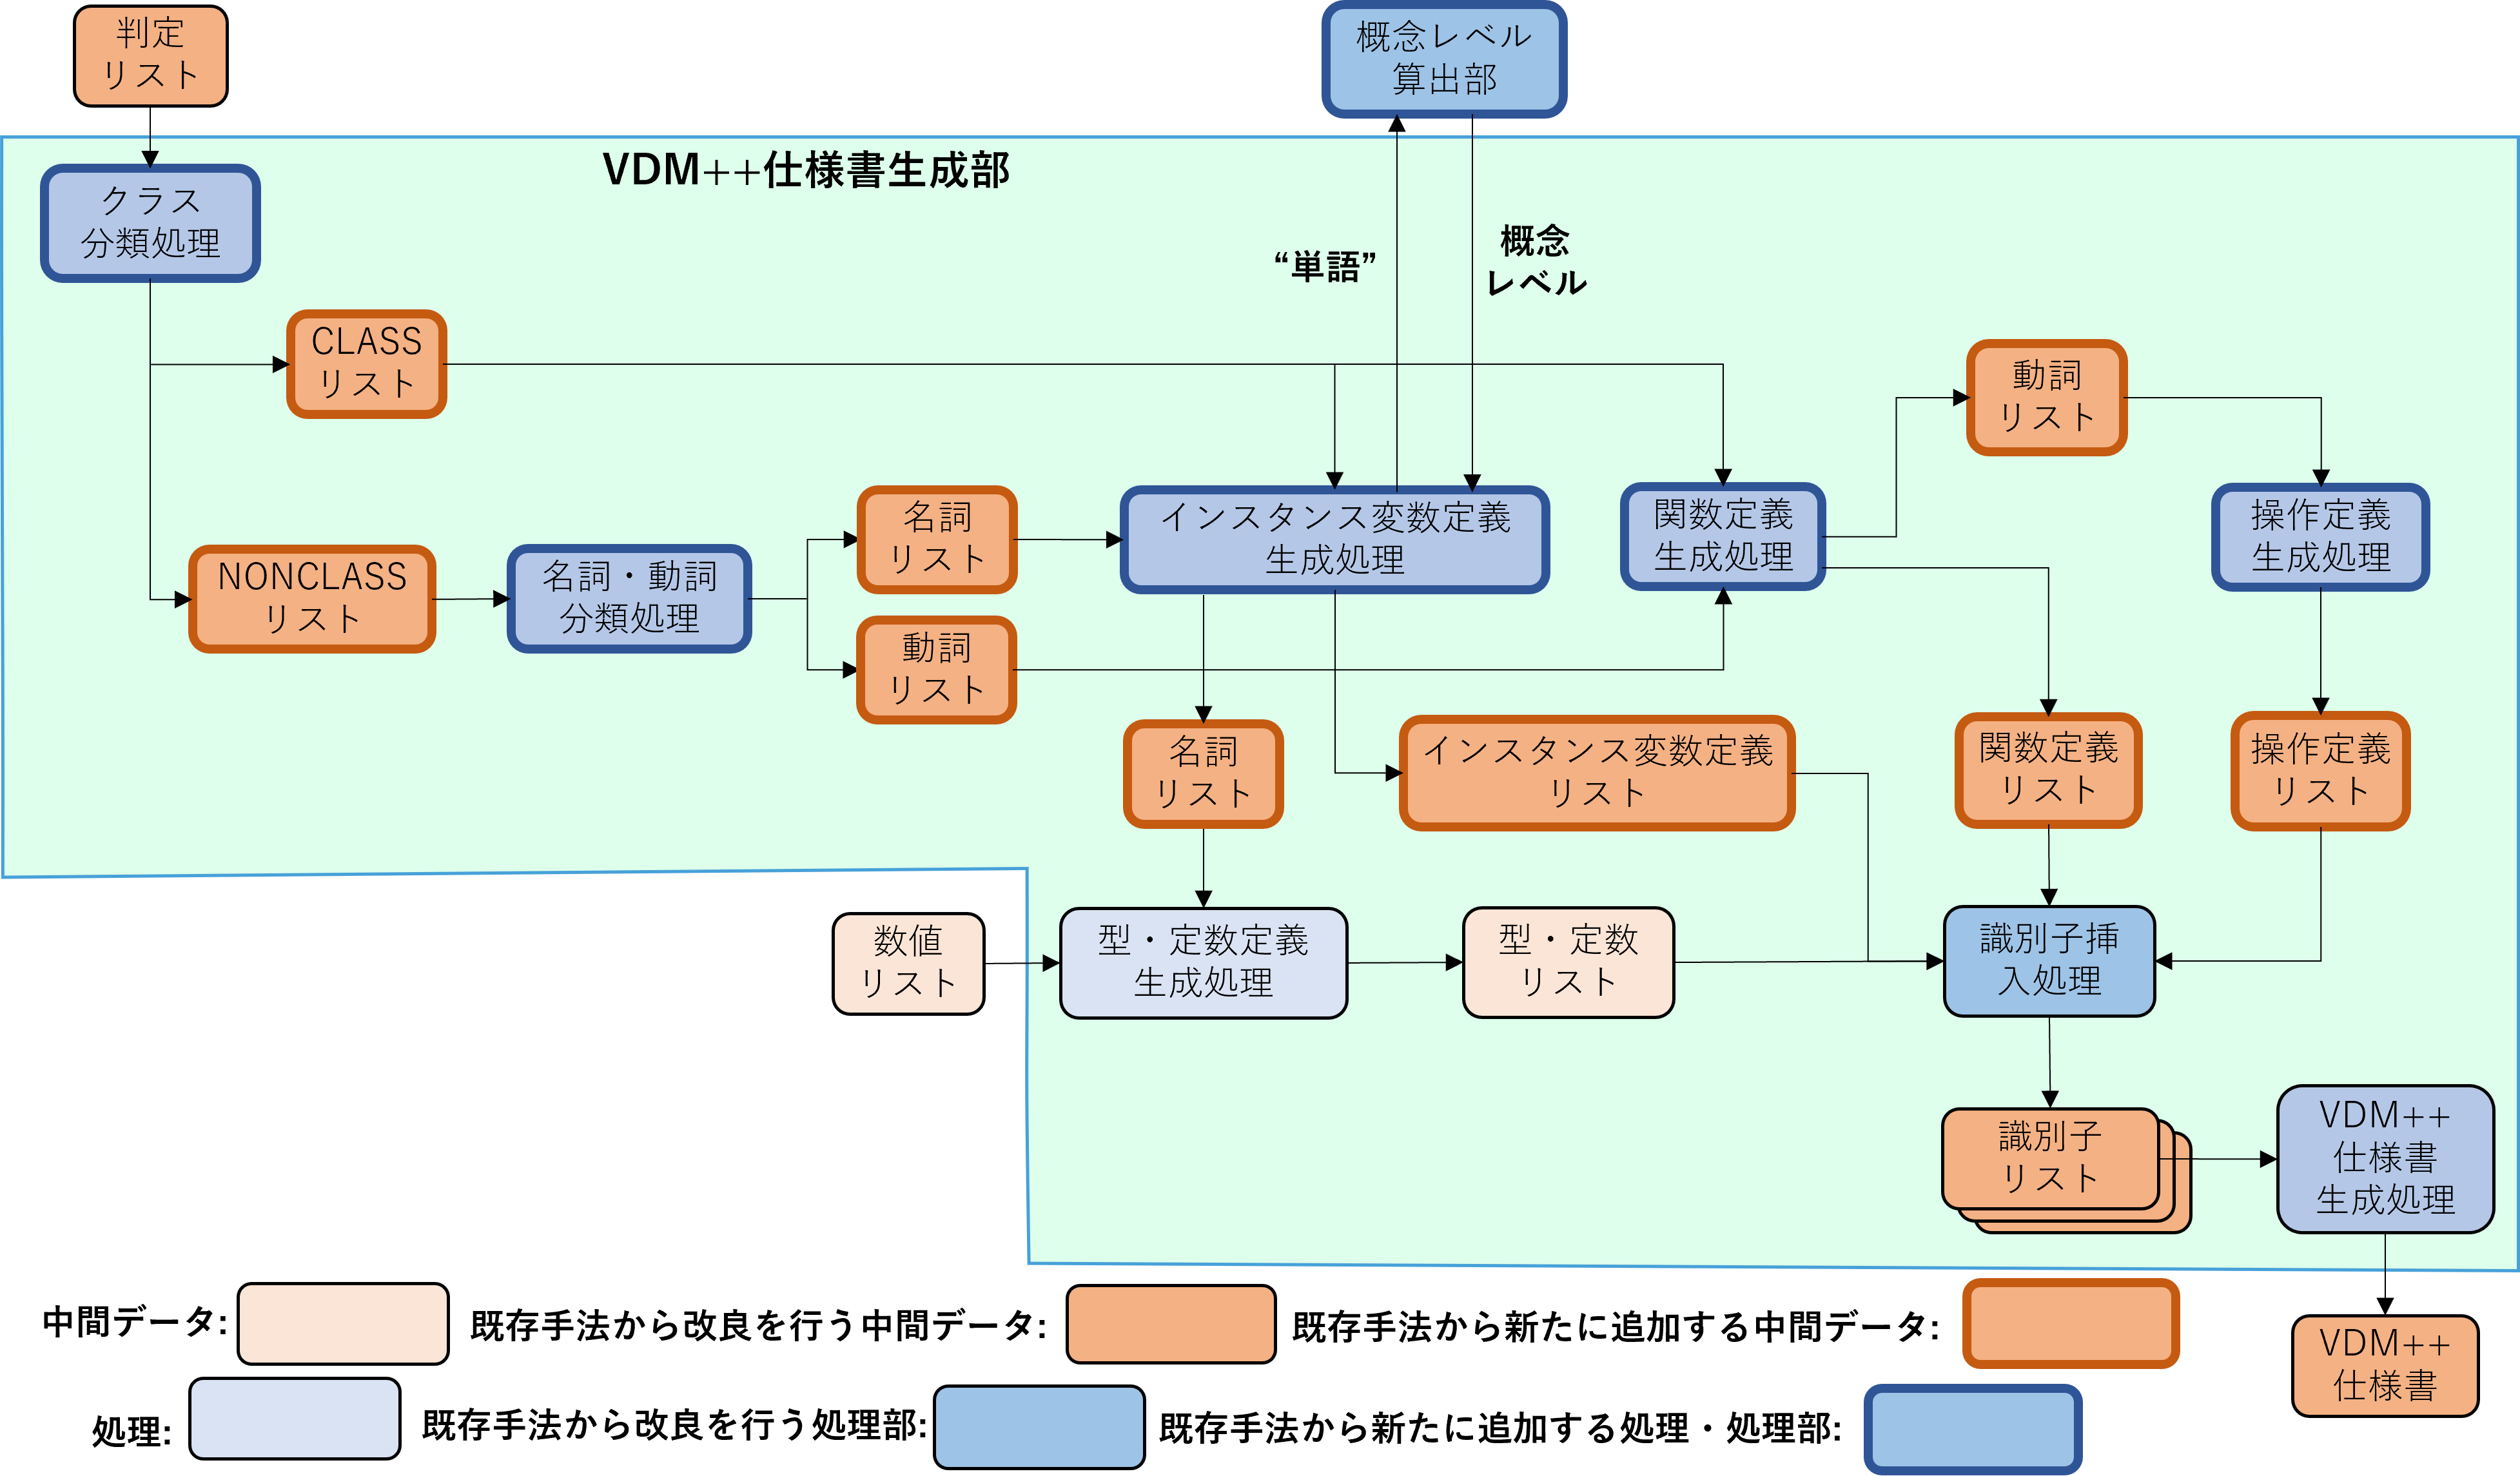
\includegraphics[width=1.0\columnwidth]{image/vgml_generator.png}
        \caption{VGMLのVDM++仕様書生成部の構造}
        \label{fig:vgml_generator}
    \end{center}
\end{figure}

\begin{figure}[t]
    \begin{center}
        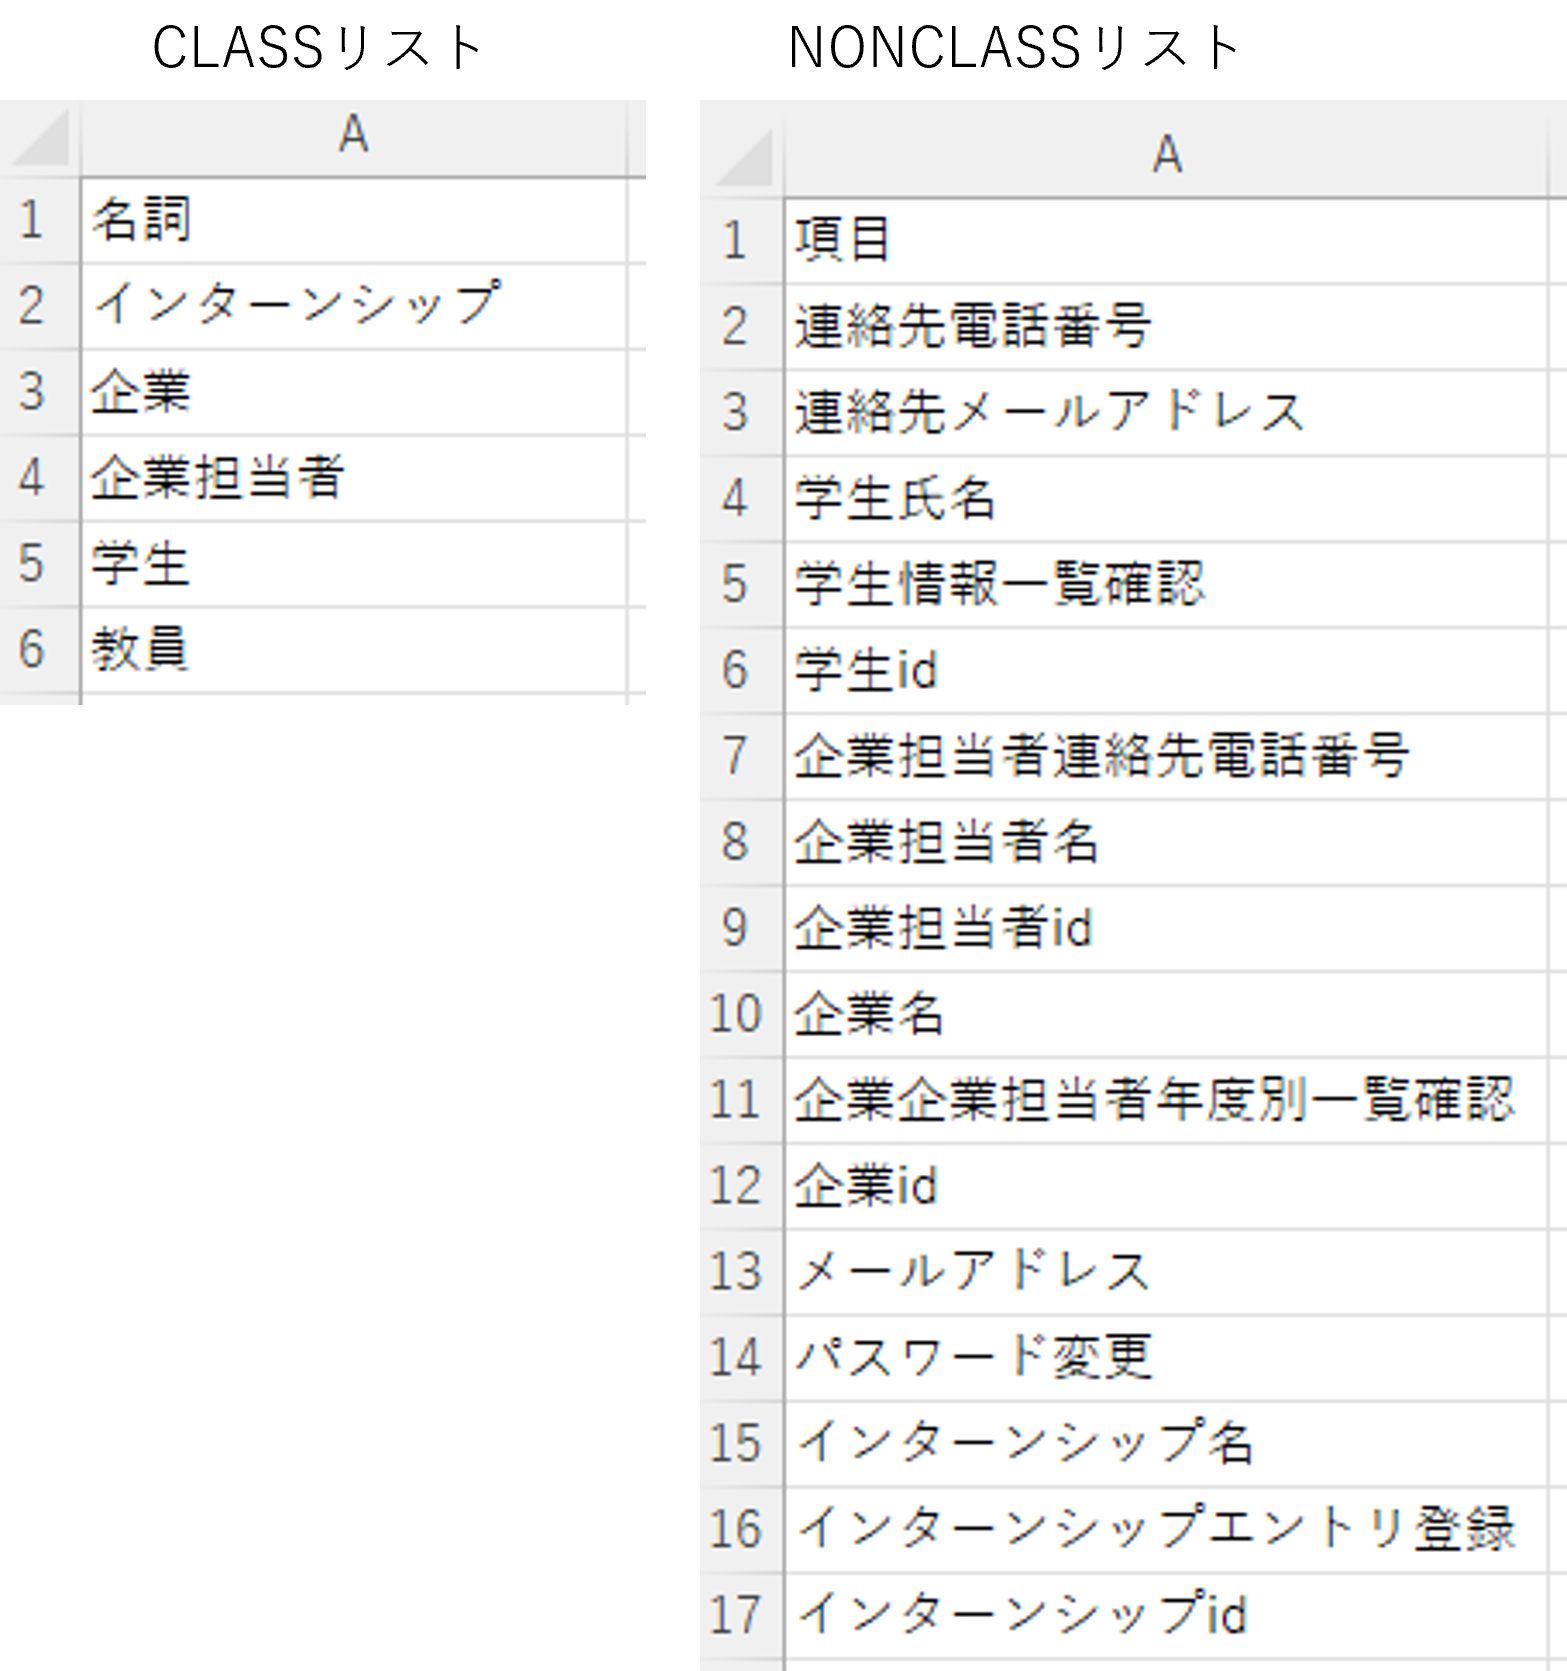
\includegraphics[width=300]{image/class_nonclass_list.png}
        \caption{CLASSリストとNONCLASSリストの例}
        \label{fig:class_nonclass_list}
    \end{center}
\end{figure}

VGMLにおけるVDM++仕様書生成部のクラス分類処理の流れを、以下に示す。

\begin{enumerate}
    \item 判定リストを入力として読み込む。
    \item 2つの空のファイルAとファイルBを用意する。
    \label{sec:class_list}
    \item 判定リストの行の数だけ、以下の処理を繰り返す。
        \begin{enumerate}
            \item 判定リストの判定結果がCLASSであった場合は、判定リストの単語を\ref{sec:class_list}で用意した空のファイルAに追加する。
            \item 判定リストの判定結果がNONCLASSであった場合は、判定リストの単語を\ref{sec:class_list}で用意した空のファイルBに追加する。
        \end{enumerate}
\end{enumerate}

\ref{sec:class_list}のファイルAとファイルBの1行は、(判定リストの単語)で構成する。
このファイルAがCLASSリスト、ファイルBがNONCLASSリストである。

\section{インスタンス変数定義を生成する処理の追加}
\label{sec:instance_generate}
本節では、自然言語仕様書からVDM++仕様書におけるインスタンス変数定義を生成する手法について説明する。
具体的には、既存手法に対して以下の処理部の追加を行う。

\begin{itemize}
    \item VDM++仕様書生成部にクラス以外の単語を名詞と動詞に分類する処理の追加
    \item VDM++仕様書生成部にインスタンス変数定義の候補である単語を抽出する処理の追加
\end{itemize}

以降、2つの追加した処理について詳細を述べる。

\subsection{単語を名詞と動詞に分類する処理の追加}
\label{sec:classifier_meishi}
VGMLは、NONCLASSリスト内の単語を、名詞である単語と動詞化できる単語に分類することによって、単語が自然言語仕様書内で振る舞いを表すか否かの判定を行う。
VGMLにおけるVDM++仕様書生成部の名詞・動詞分類処理は、NONCLASSリストを入力として、NONCLASSリスト内の単語を\ref{}節で述べたMecabを用いて形態素解析する。
さらに、名詞を表す単語を格納した名詞リストと、動詞化できる単語を格納した動詞リストを生成する。
名詞リストと動詞リストの例を、図\ref{fig:meishi_doshi_list}に示す。

\begin{figure}[t]
    \begin{center}
        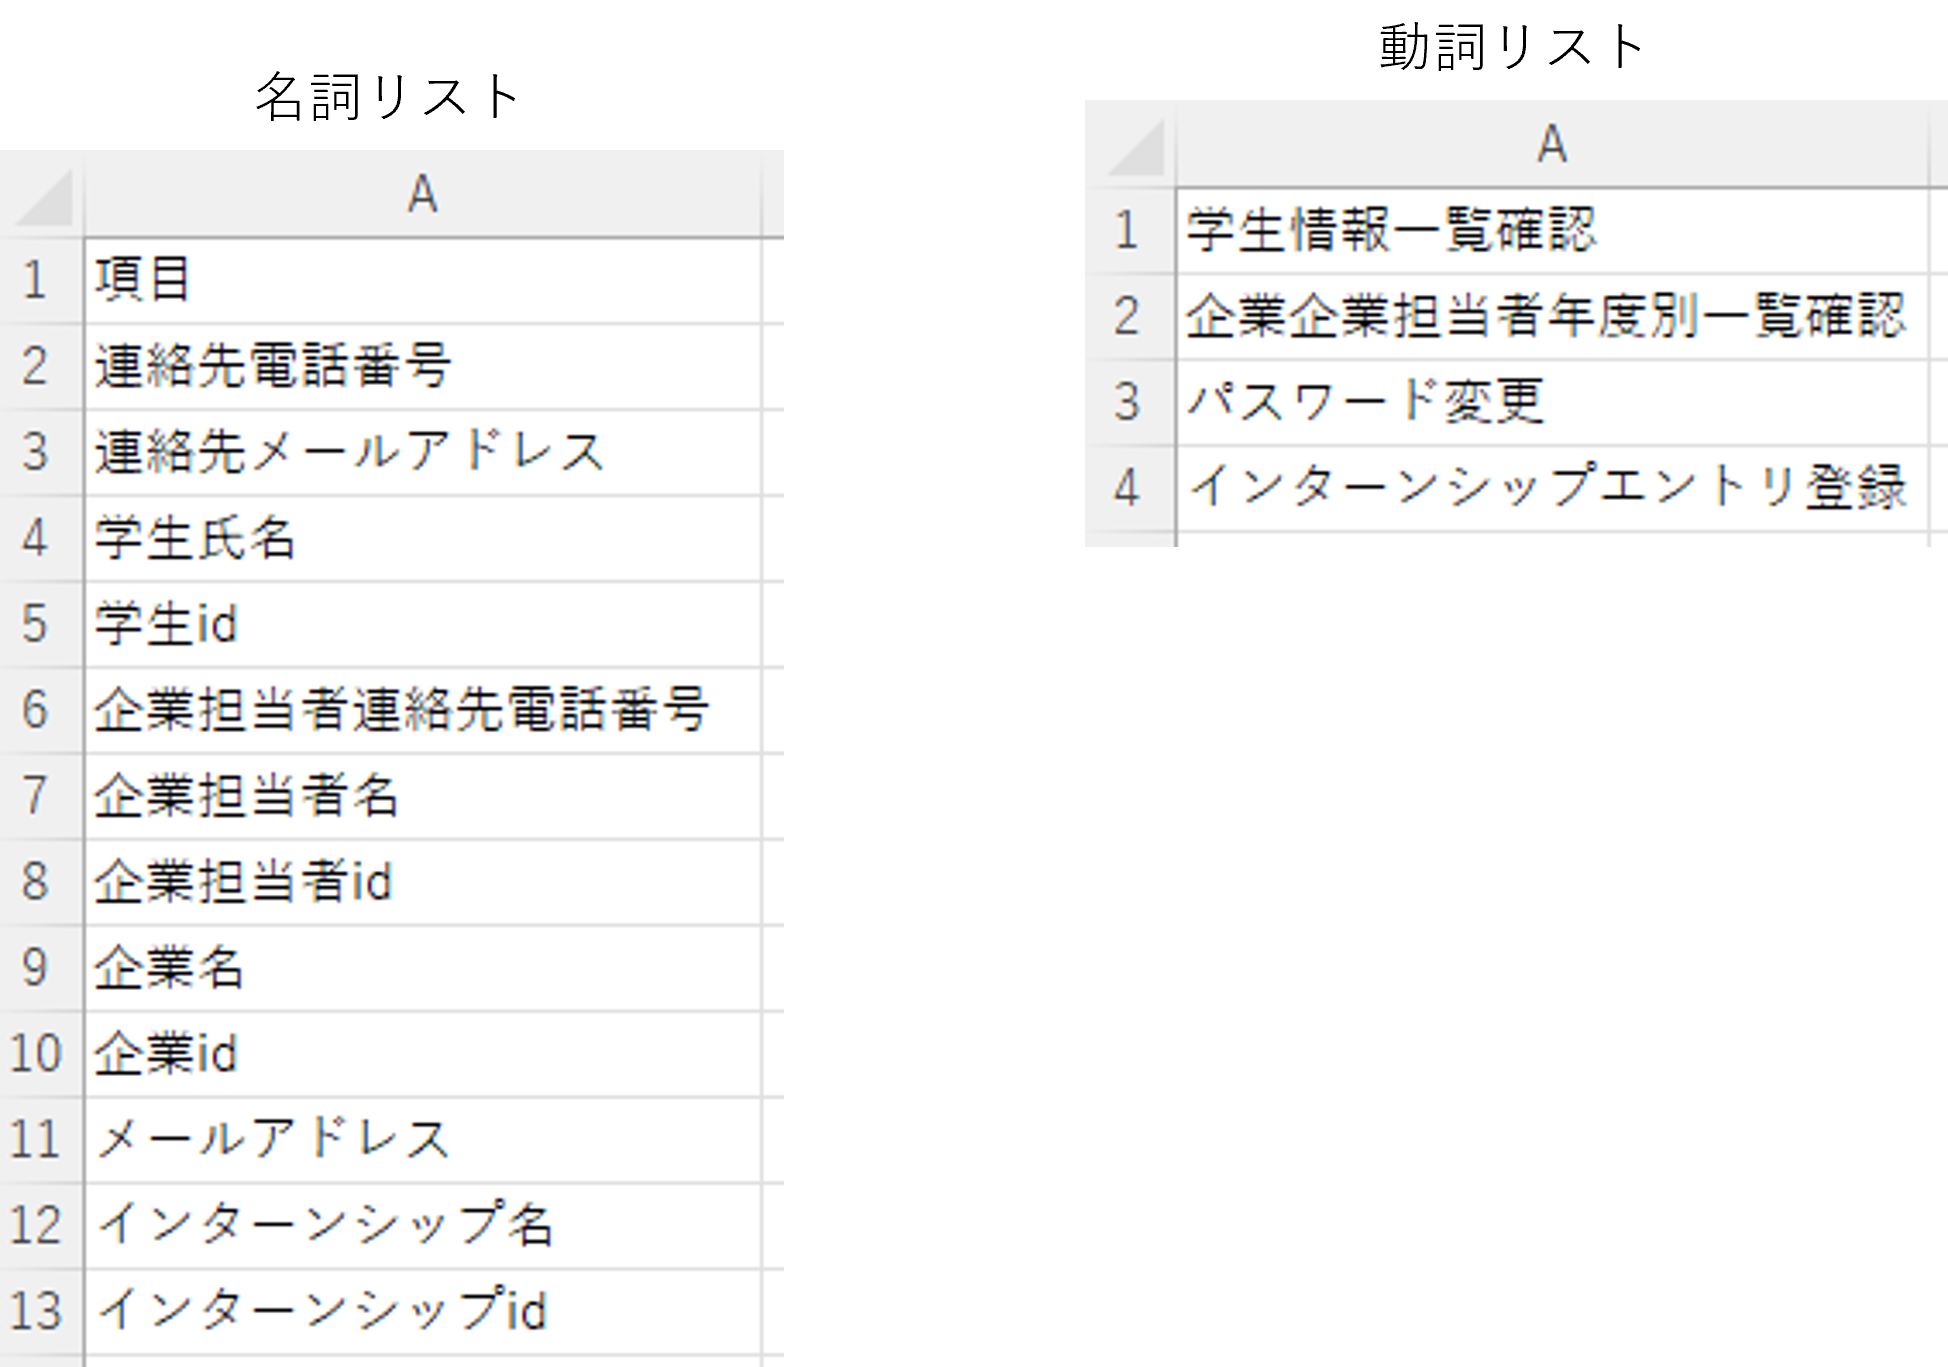
\includegraphics[width=500]{image/meishi_doshi_list.png}
        \caption{名詞リストと動詞リストの例}
        \label{fig:meishi_doshi_list}
    \end{center}
\end{figure}

VGMLにおけるVDM++仕様書生成部の名詞・動詞分類処理の流れを、以下に示す。

\begin{enumerate}
    \item NONCLASSリストを入力として読み込む。
    \item 2つの空のファイルAとファイルBを用意する。
    \label{doshi_list}
    \item NONCLASSリストの行の数だけ、以下の処理を繰り返す。
        \begin{enumerate}
            \item 空のリストを用意する。
            \label{mecab_list1}
            \item NONCLASSリストから単語を読み込む。
            \label{read_nonclass_word}
            \item \ref{read_nonclass_word}で読み込んだ単語を、Mecabを用いて分かち書きし、分かち書きした単語を\ref{mecab_list1}で用意したリストに格納する。
            \label{mecab_list2}
            \item \ref{mecab_list2}で生成したリストの、末尾の単語の品詞を、Mecabを用いて取得する。
            \label{get_nouns}
            \item \ref{get_nouns}で取得した品詞に対し、以下のいずれかの処理を行う。
                \begin{itemize}
                    \item 品詞がサ変名詞である場合、\ref{read_nonclass_word}で読み込んだ単語を、\ref{doshi_list}で用意した空のファイルAに追加する。
                    \item 品詞がサ変名詞でない場合、\ref{read_nonclass_word}で読み込んだ単語を、\ref{doshi_list}で用意した空のファイルBに追加する。
                \end{itemize}
        \end{enumerate}
\end{enumerate}

\ref{doshi_list}のファイルAとファイルBの1行は、(判定リストの単語)で構成する。
このファイルAが動詞リスト、ファイルBが名詞リストである。

\subsection{インスタンス変数定義の候補である単語を抽出する処理の追加}
\ref{sec:classifier_meishi}節で述べた名詞リスト内の単語から、インスタンス変数定義の候補である単語を抽出するために、
VDM++仕様書生成部にインスタンス変数定義生成処理を追加する。
インスタンス変数定義生成処理は、名詞リストと\ref{sec:classifier_class}節で述べたCLASSリストを入力として、名詞リストと、インスタンス変数定義リストを出力する。
インスタンス変数定義生成処理が出力する名詞リストは、入力として受け取った名詞リストの単語の内、
インスタンス変数定義の候補である単語を除いた単語を格納したリストである。
インスタンス変数定義生成処理が生成するインスタンス変数定義リストを、図\ref{fig:instance_list}に示す。

\begin{figure}[t]
    \begin{center}
        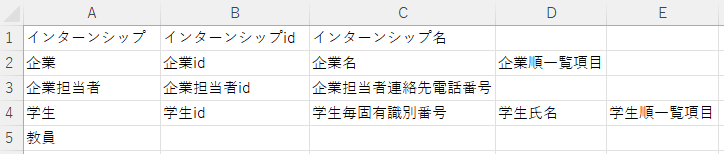
\includegraphics[width=1.0\columnwidth]{image/instance_list.png}
        \caption{インスタンス変数定義リストの例}
        \label{fig:instance_list}
    \end{center}
\end{figure}

VGMLにおけるVDM++仕様書生成部のインスタンス変数定義生成処理の流れを、以下に示す。

\begin{enumerate}
    \item CLASSリストと名詞リストを入力として読み込む。
    \item 2つの空のファイルAとファイルBを用意する。
    \label{instance_list}
    \item CLASSリストの行の数だけ、以下の処理を繰り返す。
        \begin{enumerate}
            \item CLASSリストから単語を読み込む。
            \label{class_word_for_instance}
            \item \ref{instance_list}で用意したファイルAに、\ref{class_word_for_instance}で読み込んだ単語を追加する。
            \label{instance_list2}
            \item 名詞リストの行の数だけ、以下の処理を繰り返す。
            \label{loop_meishi_list}
                \begin{enumerate}
                    \item 名詞リストから単語を読み込む。
                    \label{meishi_word}
                    \item \ref{meishi_word}で読み込んだ単語に対し、以下のいずれかの処理を行う。
                        \begin{itemize}
                            \item \ref{meishi_word}の単語が\ref{class_word_for_instance}の単語の文字列を含む場合、\ref{meishi_word}の単語の文字列から\ref{class_word_for_instance}の単語の文字列を除いた単語を生成する。
                            \label{remove_class_word}
                            \item \ref{meishi_word}の単語が\ref{class_word_for_instance}の単語の文字列を含まない、かつ、\ref{instance_list}で用意したファイルBに\ref{meishi_word}の単語が存在しない場合、ファイルBに\ref{meishi_word}の単語を追加して\ref{meishi_word}に戻る。
                            \item \ref{meishi_word}に戻る。
                        \end{itemize}
                    \item 概念レベル算出部において、\ref{class_word_for_instance}の単語の概念レベルと、\ref{remove_class_word}で生成したクラスの候補に接続する単語の概念レベルを計算する。
                    \label{calc_concept_class_meishi}
                    \item \ref{calc_concept_class_meishi}で算出した2つの単語の概念レベルの値を比較し、以下のいずれかの処理を行う。
                        \begin{enumerate}
                            \item \ref{class_word_for_instance}の単語の概念レベルの値が、\ref{remove_class_word}の単語に接続する単語の概念レベルの値より大きい場合、\ref{class_word_for_instance}で読み込んだ単語を、\ref{instance_list2}と同じ行の末尾に新たな要素として追加する。
                            \item \ref{class_word_for_instance}の単語の概念レベルの値が、\ref{remove_class_word}の単語に接続する単語の概念レベルの値より小さい、かつ、\ref{instance_list}で用意したファイルBに\ref{meishi_word}の単語が存在しない場合、\ref{instance_list}で用意したファイルBに\ref{meishi_word}の単語を追加して\ref{meishi_word}に戻る。
                            \item \ref{meishi_word}に戻る。
                        \end{enumerate}
                \end{enumerate}
        \end{enumerate}
\end{enumerate}

\ref{instance_list}のファイルAの1行は、0列目にクラスの候補である単語、1列目以降に、0列目のクラスの候補である単語が持つインスタンス変数定義の候補である単語で構成する。
このファイルが、インスタンス変数定義リストである。

\section{操作・関数定義を生成する処理の追加}
\label{sec:operate_func}
本節では、自然言語仕様書からVDM++仕様書における操作・関数定義を生成する手法について説明する。
具体的には、既存手法に対して以下の処理の追加を行う。

\begin{itemize}
    \item VDM++仕様書生成部にクラスごとに振る舞いを生成する処理の追加
    \item VDM++仕様書生成部に操作・関数定義の候補である単語を抽出する処理の追加
\end{itemize}

以降、2つの追加した処理について詳細を述べる。

\subsection{クラスごとに振る舞いを生成する処理の追加}
\label{sec:method_generator}
VGMLは、\ref{sec:classifier_meishi}節で述べた動詞リスト内の単語から、クラスごとに振る舞いを表す単語を抽出するために、
VDM++仕様書生成部に振る舞い生成処理を追加する。
振る舞い生成処理は、動詞リストと\ref{sec:classifier_class}節で述べたCLASSリスト、連結リストを入力として、振る舞いリストを生成する。
振る舞い生成処理が生成する振る舞いリストの例を、図\ref{fig:method_list}に示す。

\begin{figure}[t]
    \begin{center}
        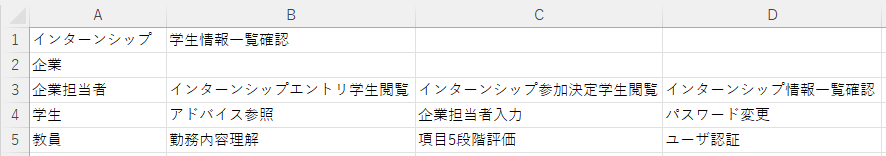
\includegraphics[width=1.0\columnwidth]{image/method_list.png}
        \caption{振る舞いリストの例}
        \label{fig:method_list}
    \end{center}
\end{figure}

VGMLにおけるVDM++仕様書生成部の振る舞い生成処理の流れを、以下に示す。

\begin{enumerate}
    \item CLASSリスト、動詞リスト、連結リストを入力として読み込む。
    \item 空のファイルを用意する。
    \label{method_list}
    \item CLASSリストの行の数だけ、以下の処理を繰り返す。
        \begin{enumerate}
            \item CLASSリストから単語を読み込む。
            \label{read_class_word}
            \item \ref{method_list}で用意したファイルに、\ref{read_class_word}の単語を追加する。
        \end{enumerate}
    \item 連結リストの行の数だけ、以下の処理を繰り返す。
    \label{loop_connect_list}
        \begin{enumerate}
            \item 連結リストから文を読み込む。
            \label{read_sentence}
            \item \ref{read_sentence}で読み込んだ文の単語の数だけ、以下の処理を繰り返す。
            \label{loop_sentence}
                \begin{enumerate}
                    \item 文から単語を読み込む。
                    \label{read_word_for_class}
                    \item ClASSリストに\ref{read_word_for_class}の単語が存在するかを検索する。
                    \label{search_class_word}
                    \item \ref{search_class_word}の検索結果に対し、以下のいずれかの処理を行う。
                        \begin{itemize}
                            \item 単語が存在しなかった場合、\ref{read_sentence}に戻る。
                            \item 単語が存在した場合、\ref{loop_sentence2}に移る。
                        \end{itemize}
                \end{enumerate}
            \item \ref{read_sentence}で読み込んだ文の単語の数だけ、以下の処理を繰り返す。
            \label{loop_sentence2}
                \begin{enumerate}
                    \item 文から単語を読み込む。
                    \label{read_word_for_method}
                    \item 動詞リストに\ref{read_word_for_method}の単語が存在するかを検索する。
                    \label{search_doshi_word}
                    \item \ref{search_doshi_word}の検索結果に対し、以下のいずれかの処理を行う。
                        \begin{itemize}
                            \item 単語が存在しなかった場合、\ref{read_sentence}に戻る。
                            \item 単語が存在した場合、\ref{read_word_for_class}の単語が存在する\ref{method_list}のファイル内の同じ行の末尾に、\ref{read_word_for_method}の単語を追加する。
                        \end{itemize}
                \end{enumerate}
        \end{enumerate}
\end{enumerate}

\ref{method_list}のファイルの1行は、1列目にクラスの候補である単語、2列目以降に、1列目のクラスの候補である単語が持つ振る舞いの候補である単語で構成する。
このファイルが、振る舞いリストである。

\subsection{操作・関数定義の候補である単語を抽出する処理の追加}
\label{sec:operate_generator}
VGMLは、\ref{sec:classifier_meishi}節で述べた振る舞いリストから、操作定義の候補である単語と、関数定義の候補である単語を抽出するために、
VDM++仕様書生成部に操作・関数定義生成処理を追加する。
操作・関数定義生成処理は、振る舞いリストと\ref{sec:classifier_class}節で述べたCLASSリストを入力として、操作定義リストと関数定義リストを出力する。
操作定義生成処理が生成する操作定義リストを図\ref{fig:operate_list}に、関数定義リストを図\ref{fig:func_list}にそれぞれ示す。
操作定義リストは、振舞いリストの振舞いを表す単語の内、クラスの候補である単語の文字列を含む単語を持つリストであり、
関数定義リストは、振舞いリストの振舞いを表す単語の内、クラスの候補である単語の文字列を含まない単語を持つリストである。

\begin{figure}[t]
    \begin{center}
        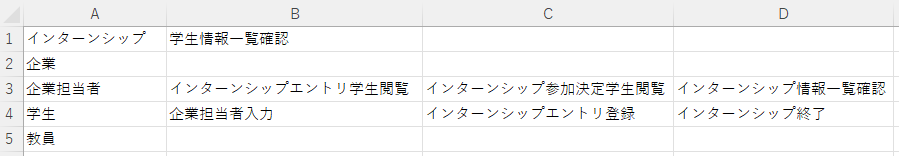
\includegraphics[width=1.0\columnwidth]{image/operate_list.png}
        \caption{操作定義リストの例}
        \label{fig:operate_list}
    \end{center}
\end{figure}

\begin{figure}[t]
    \begin{center}
        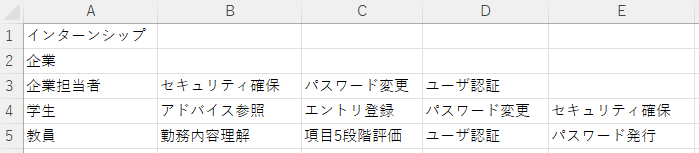
\includegraphics[width=1.0\columnwidth]{image/func_list.png}
        \caption{関数定義リストの例}
        \label{fig:func_list}
    \end{center}
\end{figure}

VGMLにおけるVDM++仕様書生成部の操作定義生成処理の流れを、以下に示す。

\begin{enumerate}
    \item 2つの空のファイルAとファイルBを用意する。
    \label{operate_list}
    \item 振舞いリストとCLASSリストを読み込む。
    \item 振舞いリストの行の数だけ、以下の処理を繰り返す。
        \begin{enumerate}
            \item 1列目のクラスの候補である単語を、\ref{operate_list}で用意したファイルAに追加する。
            \label{write_operate}
            \item 1列目のクラスの候補である単語を、\ref{operate_list}で用意したファイルBに追加する。
            \label{write_func}
            \item 2列目以降の単語の内、CLASSリスト内のいずれかの単語の文字列を含む単語を、\ref{write_operate}のファイル内の同じ行の末尾に追加する。
            \item 2列目以降の単語の内、CLASSリスト内のいずれの単語の文字列も含まない単語を、\ref{write_func}のファイル内の同じ行の末尾に追加する。
        \end{enumerate}
\end{enumerate}

\ref{operate_list}のファイルAの1行は、1列目にクラスの候補である単語、2列目以降に、1列目のクラスの候補である単語が持つ操作定義の候補である単語で構成する。
このファイルが、操作定義リストである。
\ref{operate_list}のファイルBの1行は、1列目にクラスの候補である単語、2列目以降に、1列目のクラスの候補である単語が持つ関数定義の候補である単語で構成する。
このファイルが、関数定義リストである。

\section{各定義ブロックの候補である単語をVDM++仕様書に書き込む処理の追加}
本節では、既存手法が生成する型定義と定数定義に加え、\ref{sec:generate_class}-\ref{sec:operate_func}節で述べた各定義ブロックを記述したVDM++仕様書を生成する。

具体的には、既存手法に対して以下の処理の改良を行う。

\begin{itemize}
    \item VDM++仕様書生成部の各定義ブロックの候補である単語に識別子を挿入する処理の改良。
    \item VDM++仕様書生成部のVDM++仕様書を生成する処理の改良。
\end{itemize}

以降、2つの改良した処理について詳細を述べる。

\subsection{各定義ブロックの候補である単語に識別子を挿入する処理の改良}
既存手法は、VDM++仕様書生成部の識別子挿入処理において、自然言語仕様書から抽出した単語に対し、型定義と定数定義を表す「types」と「values」のいずれかの識別子を追加する。
さらに、図\ref{}に示す識別子リストを生成する。

VGMLの識別子挿入処理は、\ref{sec:instance_generate}-\ref{sec:operate_func}節で述べたインスタンス変数定義リスト、操作定義リスト、関数定義リスト、型・定数定義リストを入力として、
既存手法が追加する「types」と「values」の識別子に加え、クラス、インスタンス変数定義、操作定義、関数定義を表す「class」、「instance variables」、「operations」、「functions」の
識別子を単語に追加できるように、識別子挿入処理を改良する。
さらに、型・定数定義識別子リストと、クラスの候補の単語の数だけクラス毎識別子リストを生成する。
ここで、型・定数定義識別子リストは、図\ref{}に示す既存手法が生成する識別子リストと同様のものである。
VGMLが生成するクラス毎識別子リストの例を、図\ref{fig:vgml_sikibetushi_list}に示す。

\begin{figure}[t]
    \begin{center}
        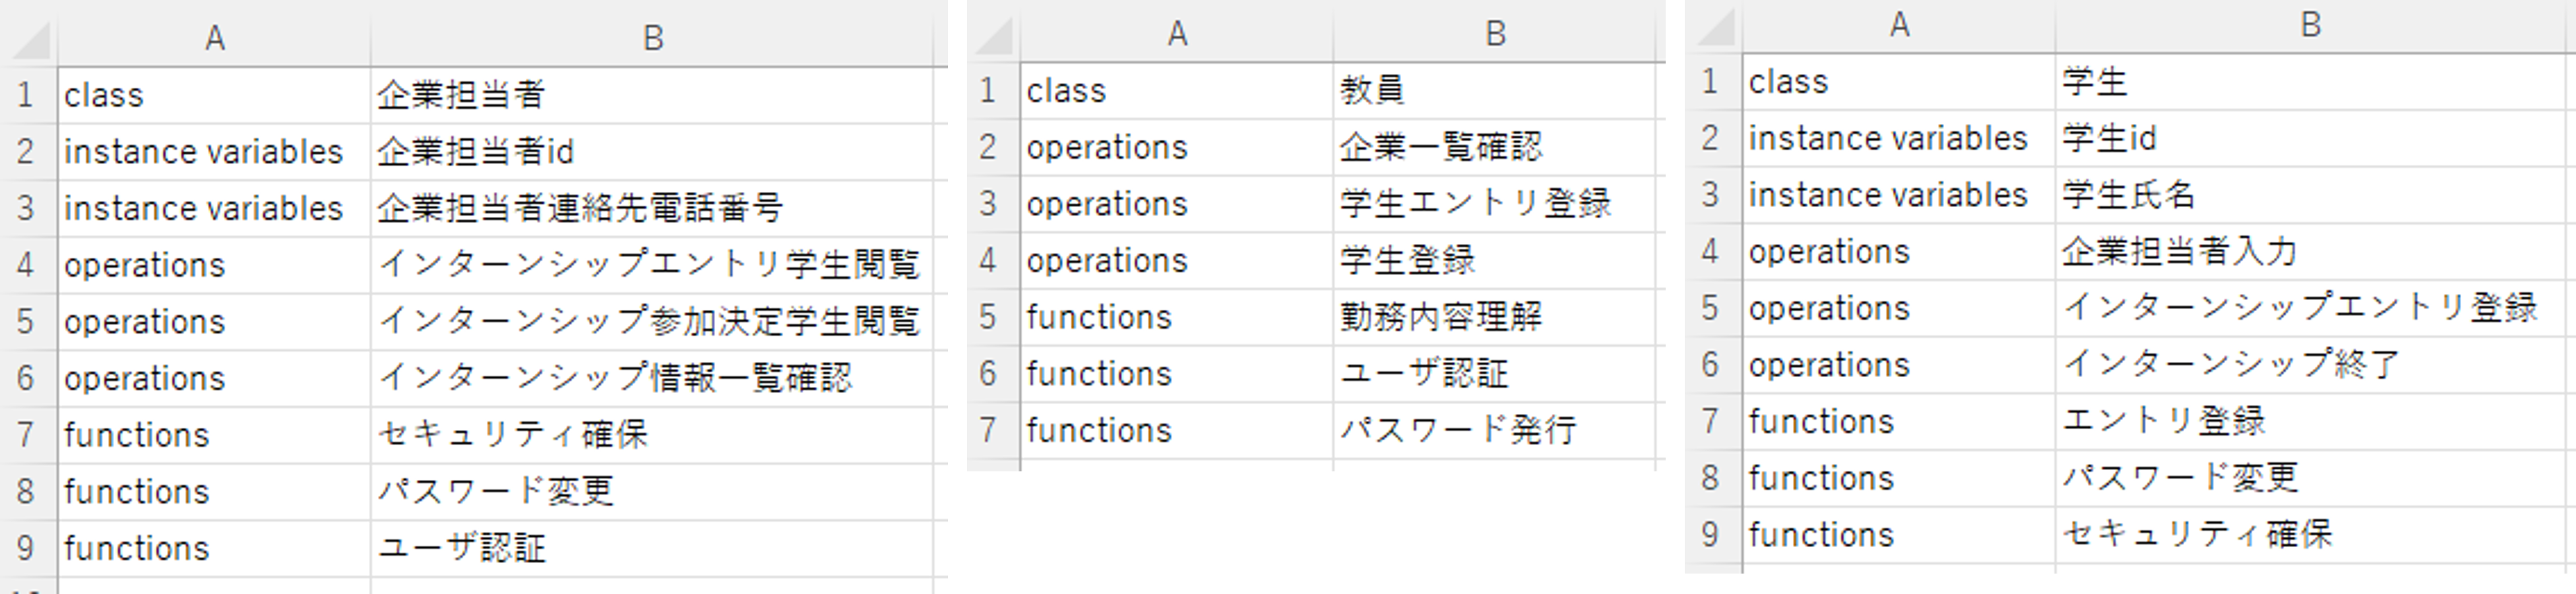
\includegraphics[width=1.0\columnwidth]{image/vgml_sikibetushi_list.png}
        \caption{クラス毎識別子リストの例}
        \label{fig:vgml_sikibetushi_list}
    \end{center}
\end{figure}

VGMLのVDM++仕様書生成部における識別子挿入処理の流れを、以下に示す。
なお、VGMLの識別子挿入処理が生成する型・定数定義識別子リストとその生成手法は、
既存手法が生成する識別子リストとその生成手法と同様のものである。
そのため、型・定数定義識別子リストを生成する処理の詳細については、説明を省略する。

\begin{enumerate}
    \item 型・定数定義リスト、インスタンス変数定義リスト、操作定義リスト、関数定義リストを入力として読み込む。
    \item 型・定数定義リストを基に、型・定数定義識別子リストを生成する。
    \item インスタンス変数定義リストの行の数だけ、以下の処理を繰り返す。
        \begin{enumerate}
            \item 空のファイルを用意する。
            \label{class_instance_list}
            \item インスタンス変数定義リストの1列目の単語を読み込む。
            \label{id_instance_word}
            \item 文字列「class」と\ref{id_instance_word}の単語を、\ref{class_instance_list}のファイルに追加する。
            \item インスタンス変数定義リストの、2列目から末尾の要素まで以下の処理を繰り返す。
                \begin{enumerate}
                    \item 当該列の単語を読み込む。
                    \label{instance_word}
                    \item 文字列「instance variables」と\ref{instance_word}の単語を、\ref{class_instance_list}のファイルに追加する。
                \end{enumerate}
        \end{enumerate}
    \item 操作定義リストの行の数だけ、以下の処理を繰り返す。
        \begin{enumerate}
            \item 操作定義リストの1列目の単語を読み込む。
            \label{id_operate_word}
            \item \ref{class_instance_list}のファイルの内、ファイルの1行1列目の単語と、\ref{id_operate_word}の単語が一致するファイルを読み込む。
            \label{class_instance_operate_list}
            \item 操作定義リストの、2列目から末尾の要素まで以下の処理を繰り返す。
                \begin{enumerate}
                    \item 当該列の単語を読み込む。
                    \label{operate_word}
                    \item 文字列「operations」と\ref{operate_word}の単語を、\ref{class_instance_operate_list}のファイルに追加する。
                \end{enumerate}
        \end{enumerate}
    \item 関数定義リストの行の数だけ、以下の処理を繰り返す。
        \begin{enumerate}
            \item 関数定義リストの1列目の単語を読み込む。
            \label{id_func_word}
            \item \ref{class_instance_list}のファイルの内、ファイルの1行1列目の単語と、\ref{id_func_word}の単語が一致するファイルを読み込む。
            \label{class_instance_operate_func_list}
            \item 関数定義リストの、2列目から末尾の要素まで以下の処理を繰り返す。
                \begin{enumerate}
                    \item 当該列の単語を読み込む。
                    \label{func_word}
                    \item 文字列「functions」と\ref{func_word}の単語を、\ref{class_instance_operate_func_list}のファイルに追加する。
                \end{enumerate}
        \end{enumerate}
\end{enumerate}

\ref{class_instance_list}のファイルは、クラスの候補の単語の数だけ生成し、1つのファイルの1行目は、(class, クラスの候補である単語名)、
2行目以降は、(instance variables,インスタンス変数定義の候補である単語名)、 (operations,操作定義の候補である単語名)、(functions,関数定義の候補である単語名)のいずれかで構成する。
このファイルが、クラス毎識別子リストである。

\subsection{VDM++仕様書を生成する処理の改良}
既存手法は、VDM++仕様書生成部のVDM++仕様書生成部において、型・定数定義識別子リスト
を入力として、図\ref{}に示す型定義と定数定義が記述したVDM++仕様書を生成する。

VGMLのVDM++仕様書生成処理は、型・定数定義識別子リストとクラス毎識別子リストを入力として、既存手法の型定義と定数定義に加え、クラス、インスタンス変数定義、操作定義、関数定義を記述した
VDM++仕様書を生成する。
VGMLが生成するVDM++仕様書の例を、図\ref{fig:4_vdm}に示す。
VGMLが生成するVDM++仕様書は、CLASSリストの要素数+1のファイルで構成する。

\begin{figure}[t]
    \begin{center}
        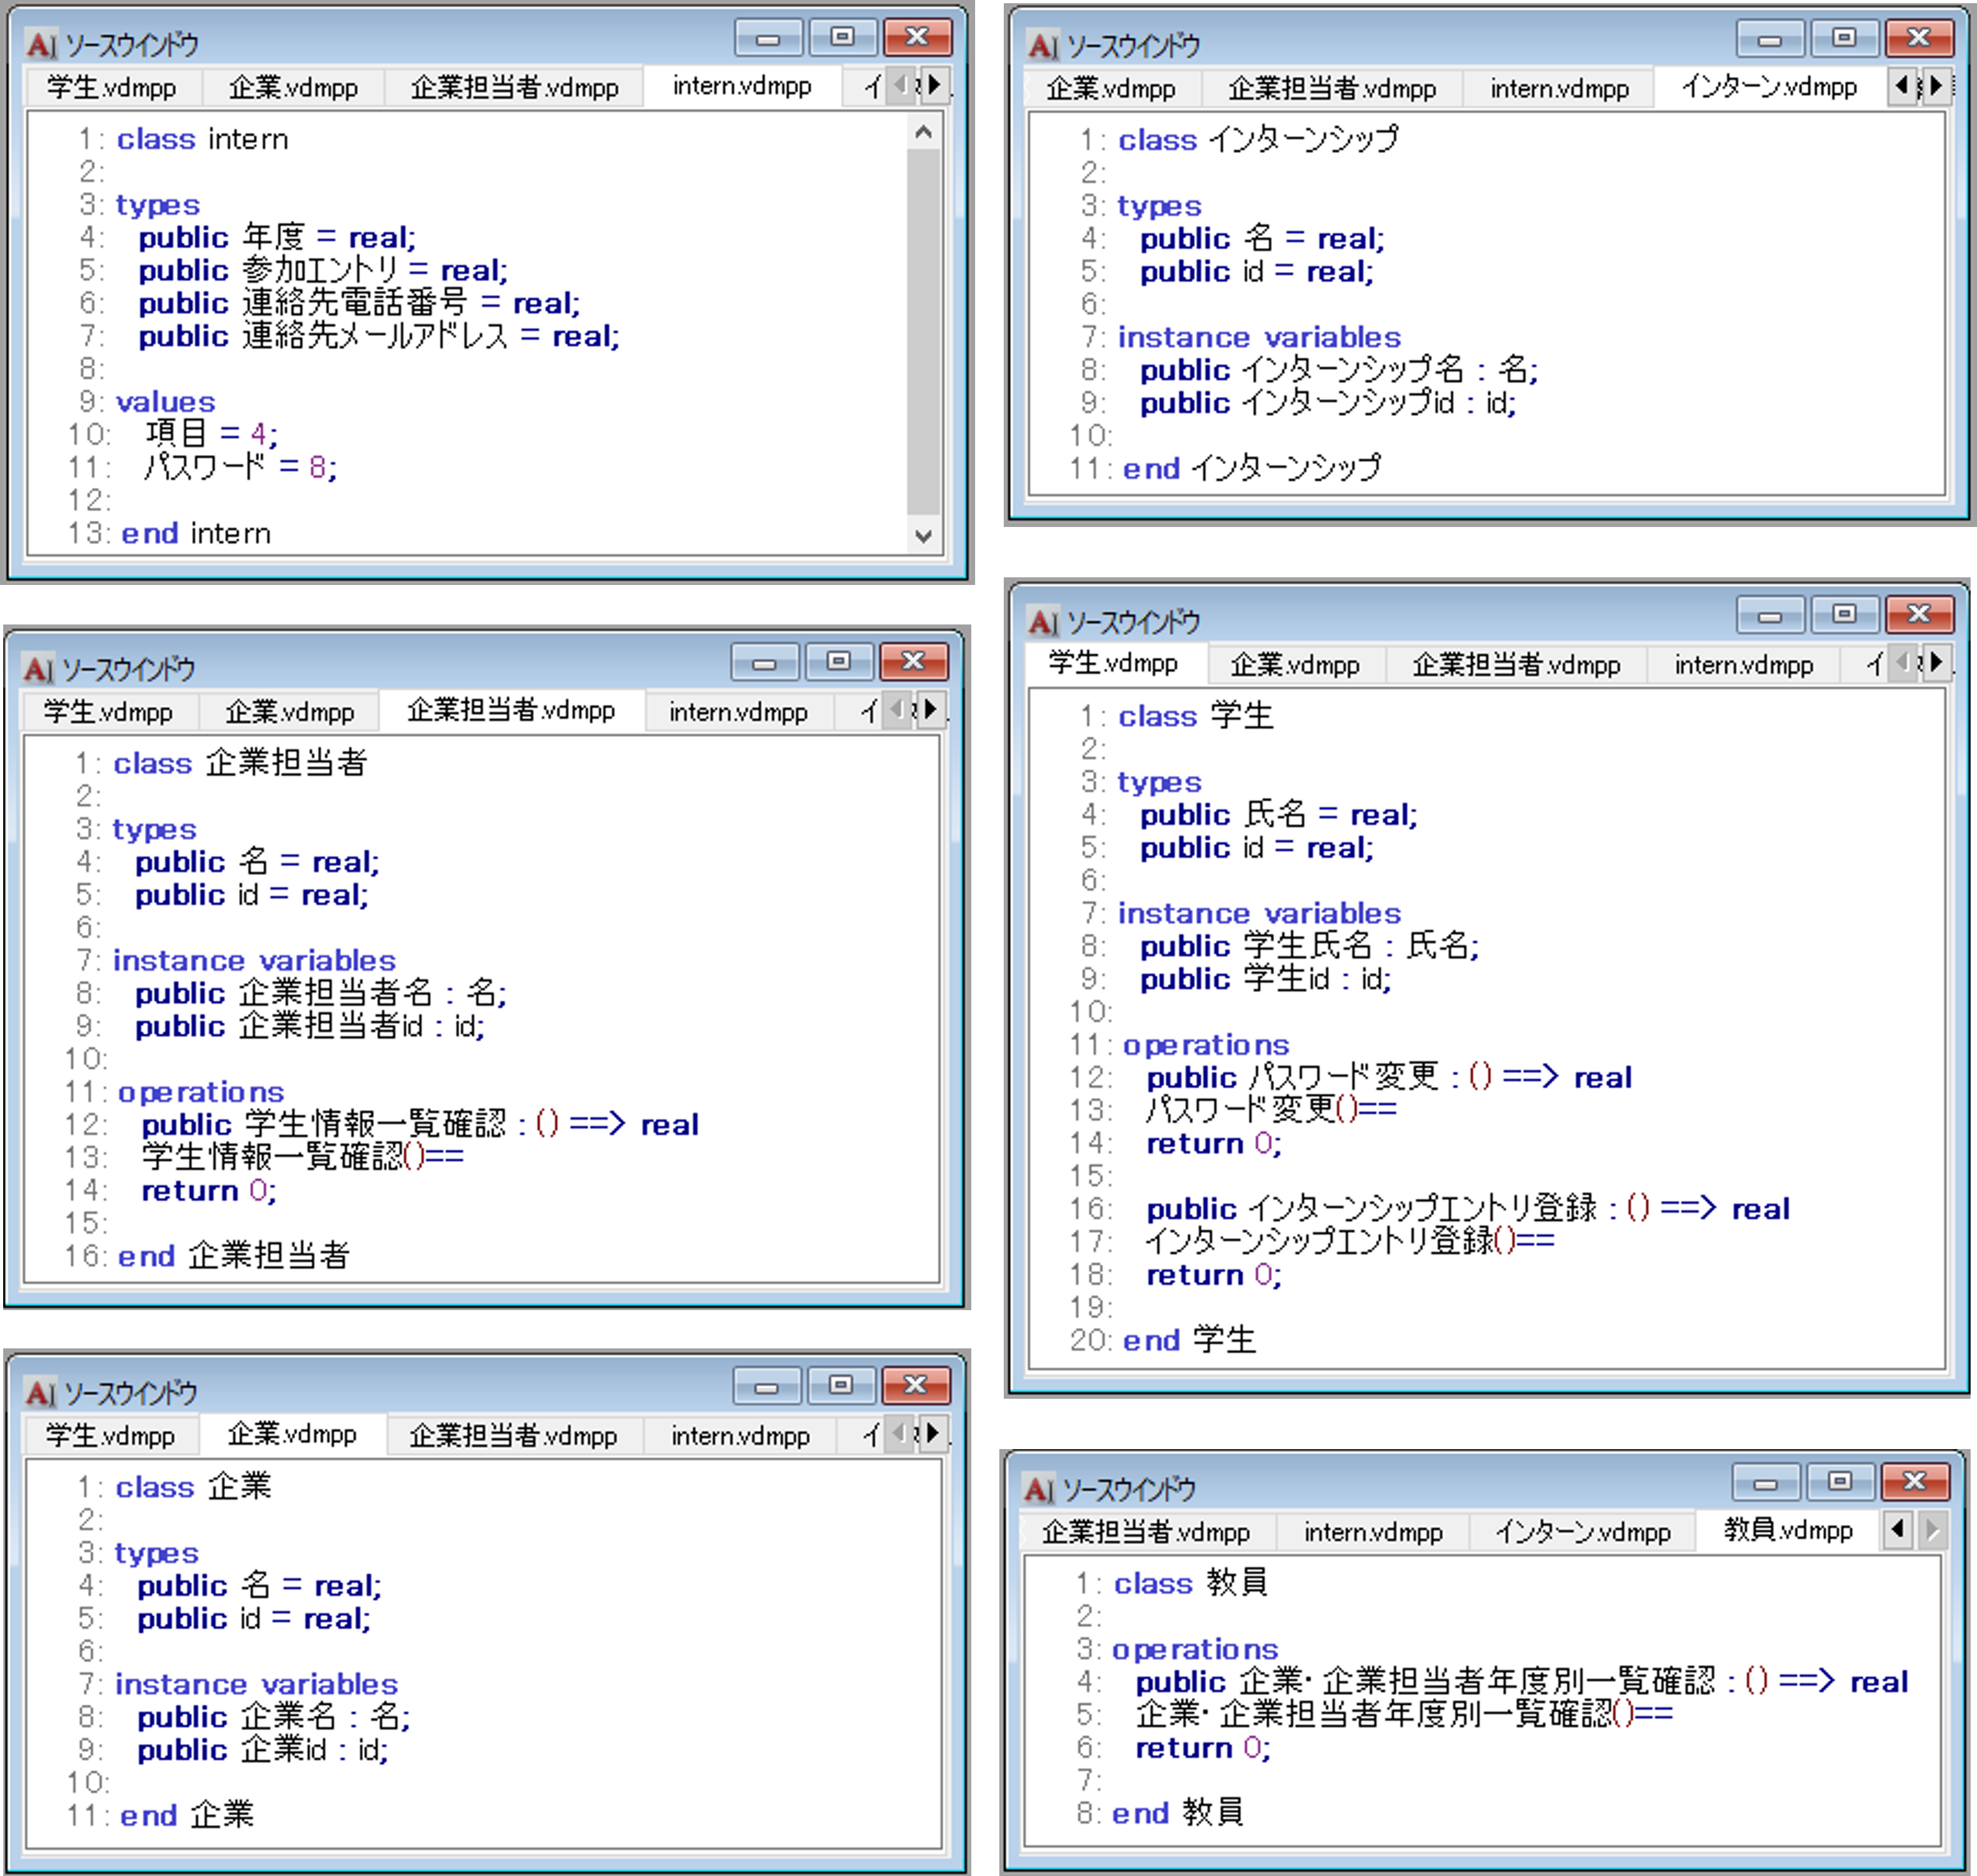
\includegraphics[width=1.0\columnwidth]{image/4_vdm.png}
        \caption{VGMLが生成するVDM++仕様書の例}
        \label{fig:4_vdm}
    \end{center}
\end{figure}

VGMLのVDM++仕様書生成部におけるVDM++仕様書生成処理の流れを、以下に示す。
なお、VGMLのVDM++仕様書生成処理が、型・定数定義識別子リストから生成するVDM++仕様書のファイルとその生成手法は、
既存手法が生成するVDM++仕様書とその生成手法と同様のものである。
そのため、型・定数定義識別子リストを基にファイルを生成する処理の詳細については、説明を省略する。
また、以下に示す処理はクラス毎識別リストの数だけ行う。

\begin{enumerate}
    \item クラス毎識別子リストと型・定数定義識別子リストを入力として読み込む。
    \item 型・定数定義識別子リストを基に、図\ref{}と同様のファイルを生成する。
    \item 空のファイルを用意する。
    \label{vdm_file}
    \item クラス毎識別子リストの1行目を読み込む。
    \label{read_class}
    \item \ref{vdm_file}で用意したファイルに、「class \textless \ref{read_class}の行の2列目の要素 \textgreater」を追加する。
    \item \ref{vdm_file}で用意したファイルに、表\ref{vdm_syntax}のVDM++の各ブロック「types」「instance variables」、「operations」、「functions」を追加する。
    \label{add_sikibetushi}
    \item クラス毎識別子リスト内の2行目以降の行に対し、以下の処理を繰り返す。
        \begin{enumerate}
            \item クラス毎識別子リストから1行読み込む。
            \label{shikibetu_elem}
            \item \ref{shikibetu_elem}の行の1列目の識別子が「instance variables」である場合、以下の処理を行う。
                \begin{enumerate}
                    \item \ref{shikibetu_elem}の行の2列目の要素である単語の文字列から、\ref{read_class}で読み込んだ行の2列目の要素である、クラスの候補である単語の文字列を除いた単語を生成する。
                    \label{read_kata}
                    \item \ref{add_sikibetushi}で追加した「types」の次の行に、表{\ref{vdm_syntax}}の構文に従って、\ref{read_kata}で生成した単語をVDM++仕様書の構文の「名前」に挿入する。
                    \item \ref{add_sikibetushi}で追加した「instance variables」の次の行に、表\ref{vdm_syntax}の構文に従って、\ref{shikibetu_elem}の行の2列目の要素をVDM++仕様書の構文の「名前」に、\ref{read_kata}で生成した単語をVDM++仕様書の構文の「型」に挿入する。
                \end{enumerate}
            \item \ref{shikibetu_elem}の行の1列目の識別子が「operations」である場合、\ref{add_sikibetushi}で追加した「operations」の次の行に、表{}の構文に従って、\ref{shikibetu_elem}の行の2列目の要素をVDM++仕様書の構文の「名前」に挿入する。
            \item \ref{shikibetu_elem}の行の1列目の識別子が「functions」である場合、\ref{add_sikibetushi}で追加した「functions」の次の行に、表{}の構文に従って、\ref{shikibetu_elem}の行の2列目の要素をVDM++仕様書の構文の「名前」に挿入する。
        \end{enumerate}
    \item \ref{vdm_file}で用意したファイルの最下行に、「end \textless \ref{read_class}の行の2列目の要素 \textgreater」を追加する。
\end{enumerate}

例として、図\ref{fig:vgml_sikibetushi_list}のファイルの内、「企業担当者」クラスを記述したファイルの、1行目、2行目、4行目、7行目について説明する。

1行目について説明する。2列目の単語を読み取る。「class」の構文「class 名前」が、2列目の「企業担当者」を「名前」に関連付ける。
そして、空のファイルを生成し、「class 企業担当者」を挿入する。

次に、2行目について説明する。1列目の識別子を読み取り、「instance variables」の次の行に記述する。
「instance variables」の構文「public 名前 : 型;」が、2列目の「企業担当者id」を「名前」に関連付ける。
さらに、「企業担当者id」から、1行2列目の「企業担当者」を除いた「id」を生成し、「id」を「型」に関連付ける。
そして、VDM ++仕様書のブロック「instance variables」の次の行に「public  = 企業担当者id : id;」を挿入する。

次に、4行目について説明する。1列目の識別子を読み取り、「operations」の次の行に記述する。
「operations」の構文「名前 : ()==\textgreater real \textless 改行 \textgreater 名前()== \textless 改行 \textgreater return 0;」が、2列目の「インターンシップエントリ学生閲覧」を「名前」に関連付ける。
そして、VDM ++仕様書のブロック「operations」の次の行に「インターンシップエントリ学生閲覧 : ()==\textgreater real \textless 改行 \textgreater インターンシップエントリ学生閲覧()== \textless 改行 \textgreater return 0;」を挿入する。

次に、7行目について説明する。1列目の識別子を読み取り、「functions」の次の行に記述する。
「functionss」の構文「名前 : ()-\textgreater real \textless 改行 \textgreater 名前()== 0;」が、2列目の「セキュリティ確保」を「名前」に関連付ける。
そして、VDM ++仕様書のブロック「functions」の次の行に「セキュリティ確保 : ()-\textgreater real \textless 改行 \textgreater セキュリティ確保()== 0;」を挿入する。